% Chapter Template

\chapter{Experiments} % Main chapter title

\label{Chapter3} % Change X to a consecutive number; for referencing this chapter elsewhere, use \ref{ChapterX}

\lhead{Chapter 3. \emph{Experiments}} % Change X to a consecutive number; this is for the header on each page - perhaps a shortened title

%----------------------------------------------------------------------------------------
%	SECTION 1
%----------------------------------------------------------------------------------------
\section{Experimental Setup}

To simulate a fat-tree topology as seen in data center networks, 4 physical servers and 2 data plane programmable switches were used. Each switch
was virtualized to create 5 switches using 10G loopback links. So, we have 10 switches in total, with 4 of them as top-of-rack or edge switches,
4 of them as aggregate switches, and 2 as core switches (Figure \ref{fig:Topology})

\begin{figure}[htbp]
	\centering
		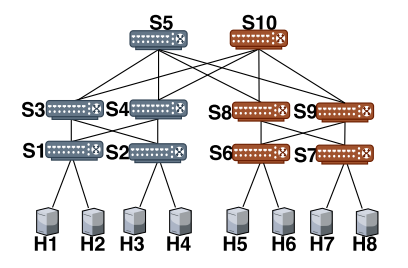
\includegraphics{Figures/Topology.png}
		\rule{35em}{0.5pt}
	\caption[Evaluation Topology]{Evaluation Topology}
	\label{fig:Topology}
\end{figure}
The rest of this chapter is structured as follows: For a potential fault that can occur in the network, we have
\begin{itemize}
    \item A section on the description of the fault
    \item A section on the configuration of switches and hosts for reproducing the fault
    \item A section on how the proposed fault can be diagnosed using SQL queries
    \item Results and relevant illustrations
\end{itemize}

The last section presents a unified scheme for diagnosing faults in networks that has been built on logic that was developed
in preceding sections. It also proposes further work to be done till the end of the semester.
\section{The Synchronous Incast Problem}

\subsection{Description}

This type of problem occurs in data centers in applications like MapReduce and DFS exhibiting fan-in traffic patterns.
This occurs when multiple hosts send data to a single host. In the case where the traffic from multiple hosts is
synchronized(common in scatter-gather architectures, Figure \ref{fig:Synch Incast}), it may lead to heavy congestion for a short duration (of the
order of microseconds) and lead to spikes in queuing delay even when none of the flows are individually anywhere near
the capacity of the link.

\begin{figure}[htbp]
	\centering
		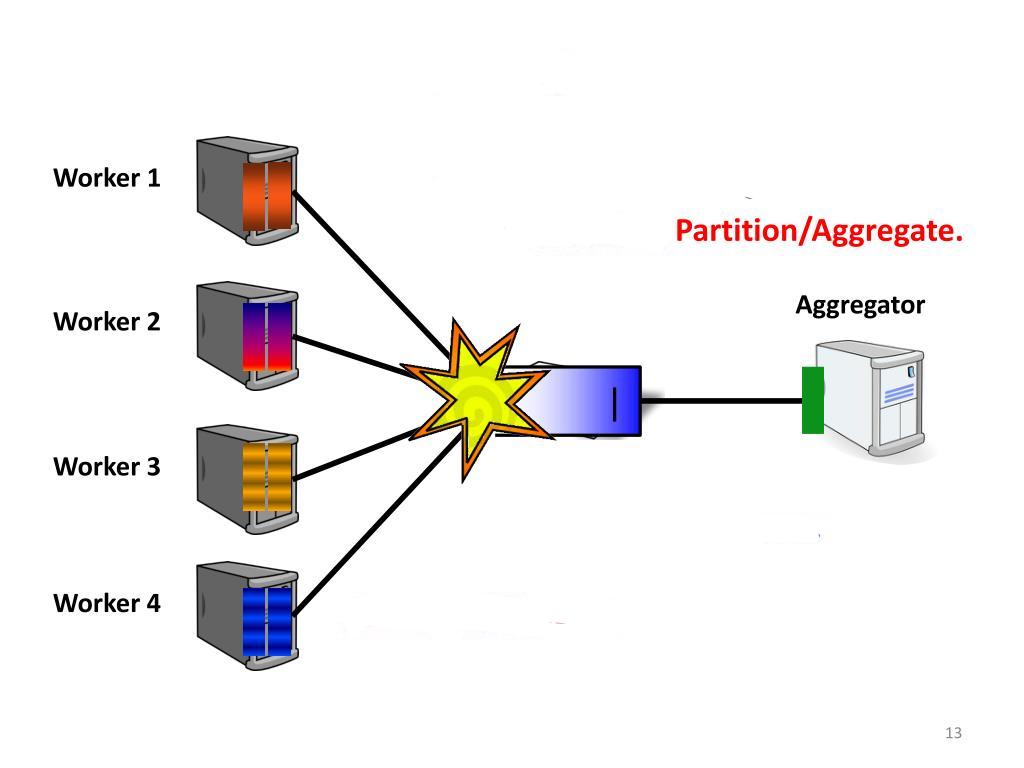
\includegraphics[width=0.65\columnwidth]{Figures/sync_incast.jpg}
		\rule{35em}{0.5pt}
	\caption[Synchronized Incast]{Synchronized Incast in Partition-Aggregate architecture}
	\label{fig:Synch Incast}
\end{figure}

\subsection{Configuration}
For creating a synchronized incast scenario in our topology, we generate traffic of 1 Gbps from hosts H1 to H6. The flow are routed
according to Figure \ref{fig:Synch Incast Topo} and get aggregated at switch 7.
\begin{figure}[htbp]
	\centering
		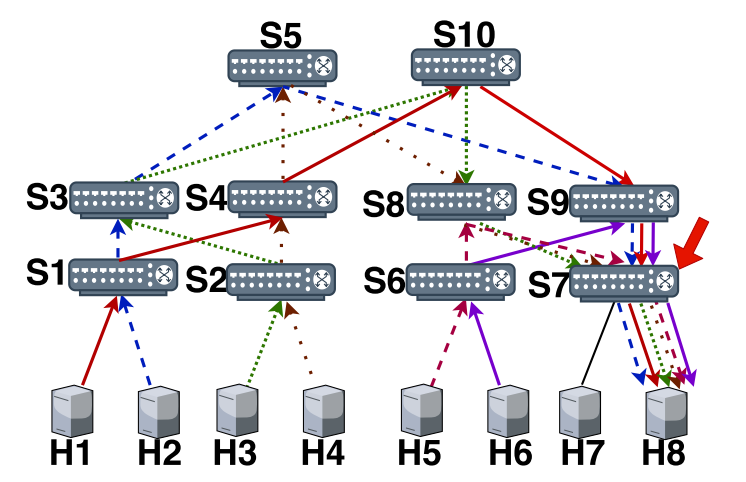
\includegraphics[width=0.65\columnwidth]{Figures/sync_incast_topo.png}
		\rule{35em}{0.5pt}
	\caption[Synchronized Incast Flows]{Synchronized Incast at switch 7 due to synchronized Fan-in traffic}
	\label{fig:Synch Incast Topo}
\end{figure}


\subsection{Diagnosis}
A synchronized microburst will often lead to multiple spikes occuring in a plot 
of the queue depth at the trigger switch. An algorithm for determining the width of
the peak queueDepth is described here.

\begin{algorithm}
	\caption{Estimate Width of Peak}
	\begin{algorithmic}[1]
		\REQUIRE indexOfPeak, records, peakDepth
		\STATE $leftThreshold \leftarrow 0.3, rightThreshold \leftarrow 0.5$
		\STATE $leftIndex = indexOfPeak - 1$
		\STATE $rightIndex = indexOfPeak + 1$
		% \WHILE{$leftIndex \geq 0$}
		
		\WHILE{$records[leftIndex].depth \geq leftThreshold \times peakDepth$}
		\STATE $leftIndex = leftIndex - 1$
		\ENDWHILE

		\WHILE{$records[rightIndex].depth \geq rightThreshold \times peakDepth$}
		\STATE $rightIndex = rightIndex + 1$
		\ENDWHILE

		\STATE $width = records[rightIndex].timeOut - records[leftIndex].timeIn$
		% \ENDWHILE
		% }
	\end{algorithmic}
\end{algorithm}

Once the peak is estimated, we look at the distribution of packets that came into the queue during the peak
as well as the packets that were present in the queue at the start of the peak.
We use Jain's Fairness Index (Appendix \ref{AppendixA}) to estimate fairness of distribution of packets according to source IP.
If the Jain's Fairness Index turns out to be greater than a predetermined threshold of 0.7, then it is classified as a case of 
Synchronized Incast due to the observation that in a synchronized incast, the distribution of packets is mostly fair.
\subsection{Results and Illustrations}
The above heuristic was applied in 5 different scenarios of synchronized incast of varied transmission rates.
The resultant values of Fairness Index calculated are given in table \ref{tab:J_Index_Sync}
\begin{table}[h]
\begin{center}
\begin{tabular}{ |p{3cm}|p{3cm}|  }
	\hline
	\multicolumn{2}{|c|}{Jain's Index} \\
	\hline
	Scenario & Value \\
	\hline
	1 & 0.957 \\
	2 & 0.980 \\
	3 & 0.890 \\
	4 & 0.780 \\
	5 & 0.975 \\
	\hline
   \end{tabular}
\end{center}

\caption{Jain's Index Values for different scenarios of Synchronous Incast}
% Help
\label{tab:J_Index_Sync}
\end{table}

Further, to help the network operator visualize the scenario, plots of link utilization and queue depth at 
trigger switch are plotted, along with packet distribution in the estimated peak, as shown in figures \ref{fig:link_utilization_sync}, \ref{fig:queue_depth_sync}
and \ref{fig:distribution_sync}

\begin{figure}[htbp]
	\centering
		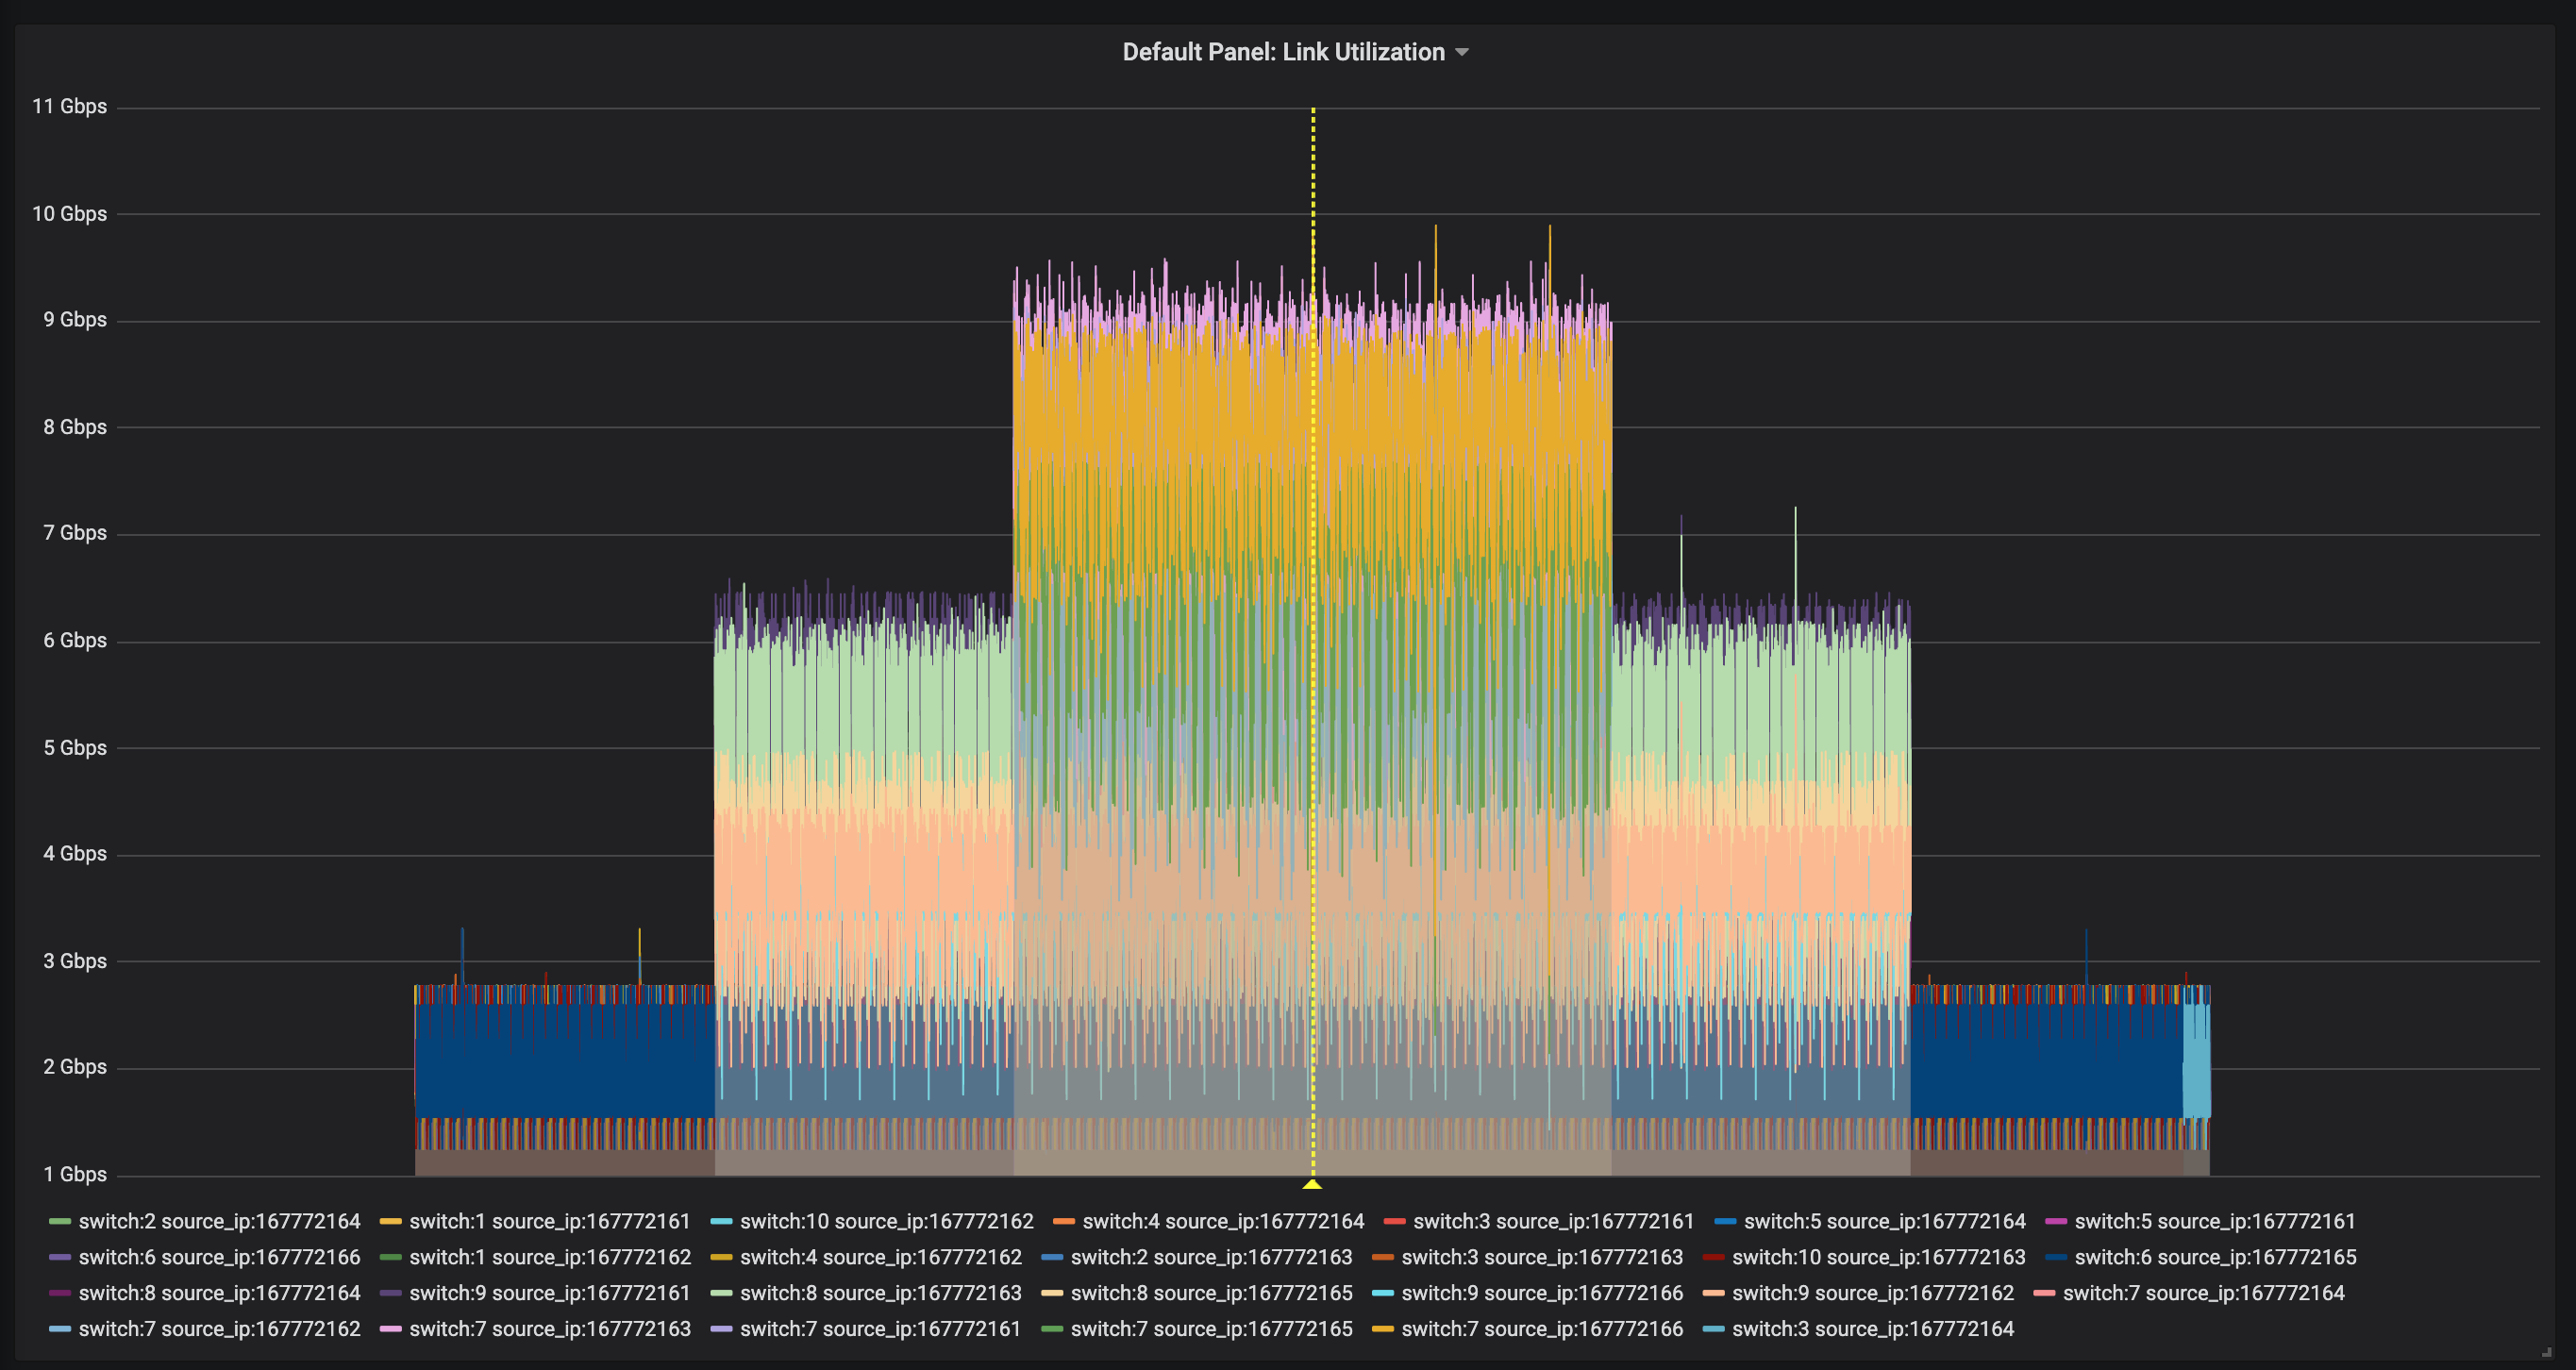
\includegraphics[width=1.0\columnwidth]{Figures/link_utilization_sync.png}
		\rule{35em}{0.5pt}
	\caption[Link Utilization at Trigger Switch, Sync Incast]{Link Utilization at Trigger Switch, Sync Incast}
	\label{fig:link_utilization_sync}
\end{figure}
\begin{figure}[htbp]
	\centering
		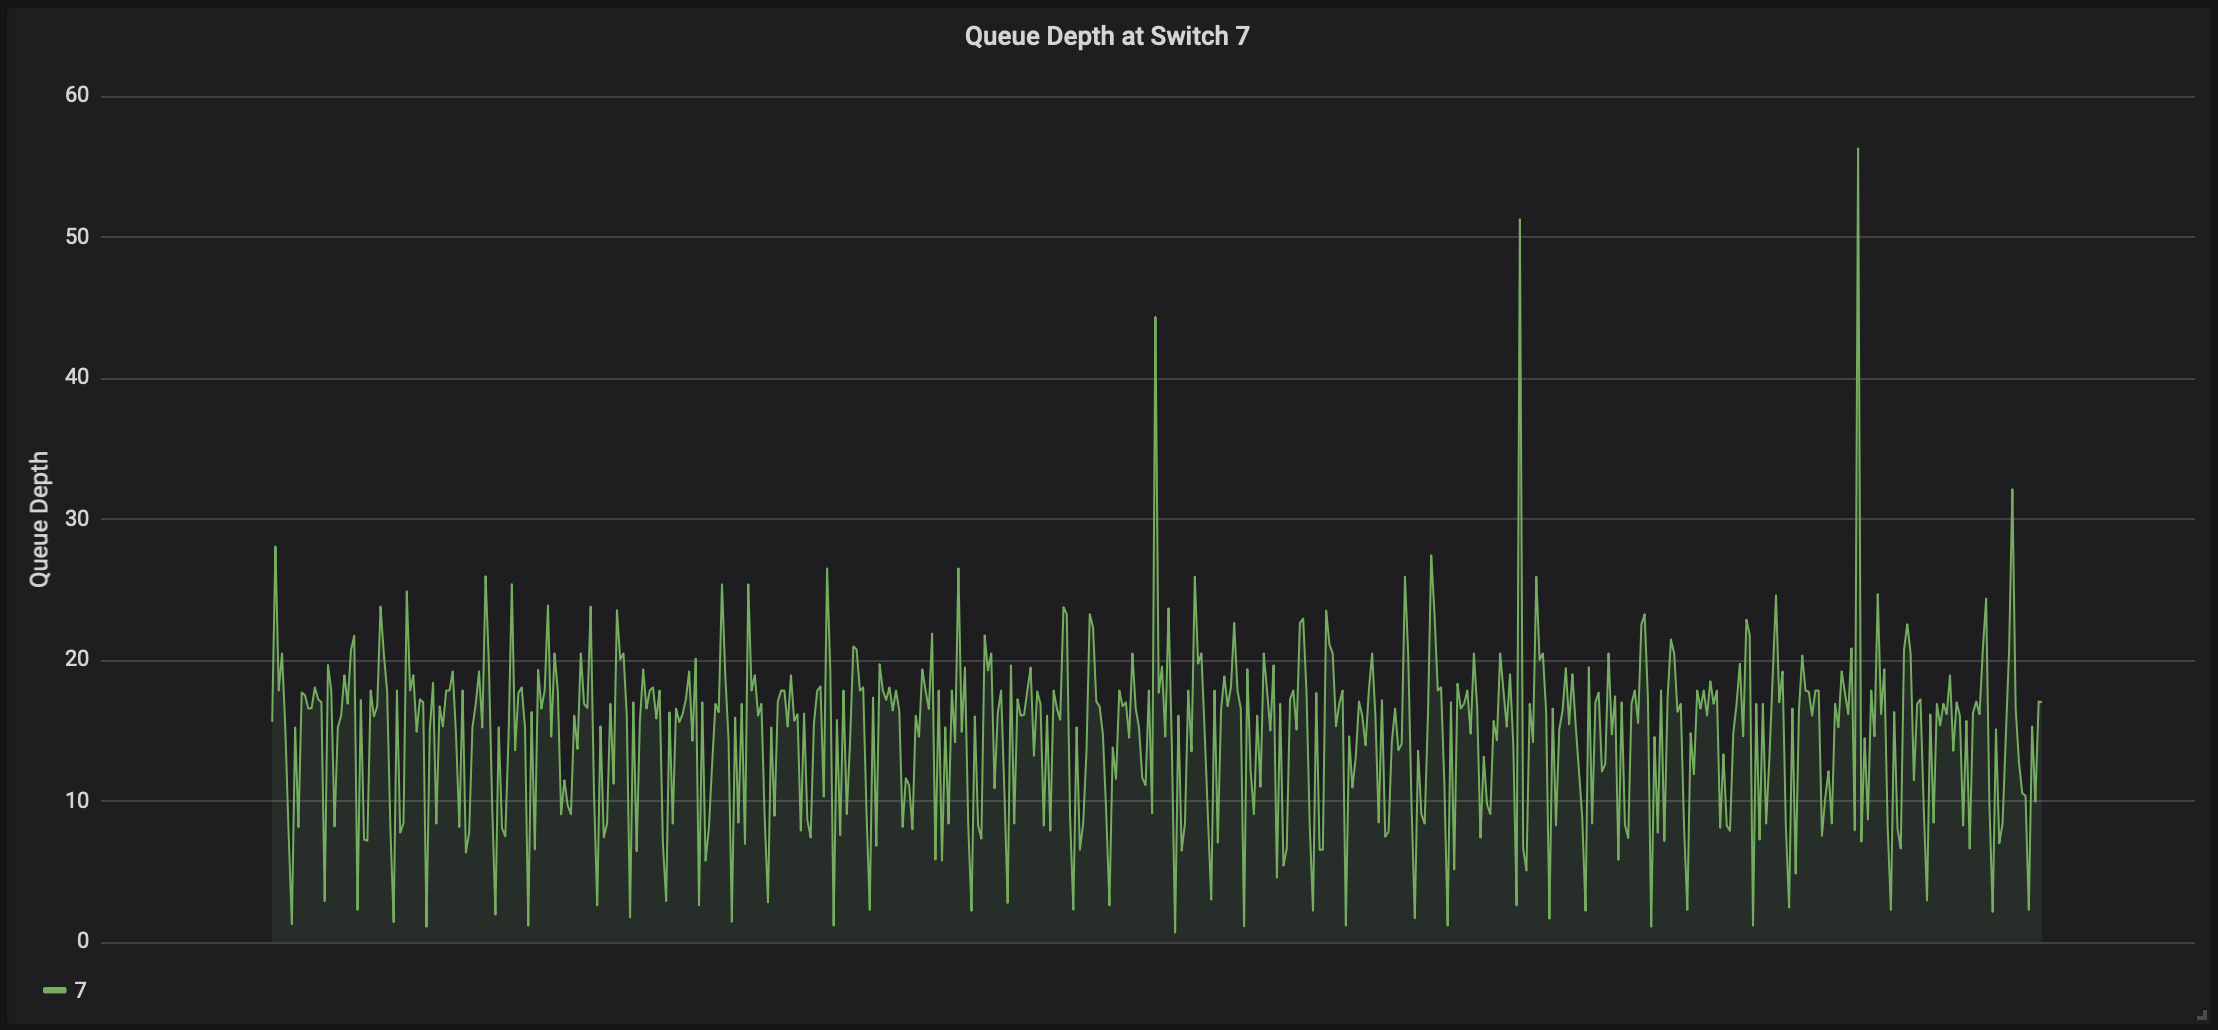
\includegraphics[width=1.0\columnwidth]{Figures/queue_depth_sync.png}
		\rule{35em}{0.5pt}
	\caption[Queue Depth at Trigger Switch, Sync Incast]{Queue Depth at Trigger Switch, Sync Incast}
	\label{fig:queue_depth_sync}
\end{figure}
\begin{figure}[htbp]
	\centering
		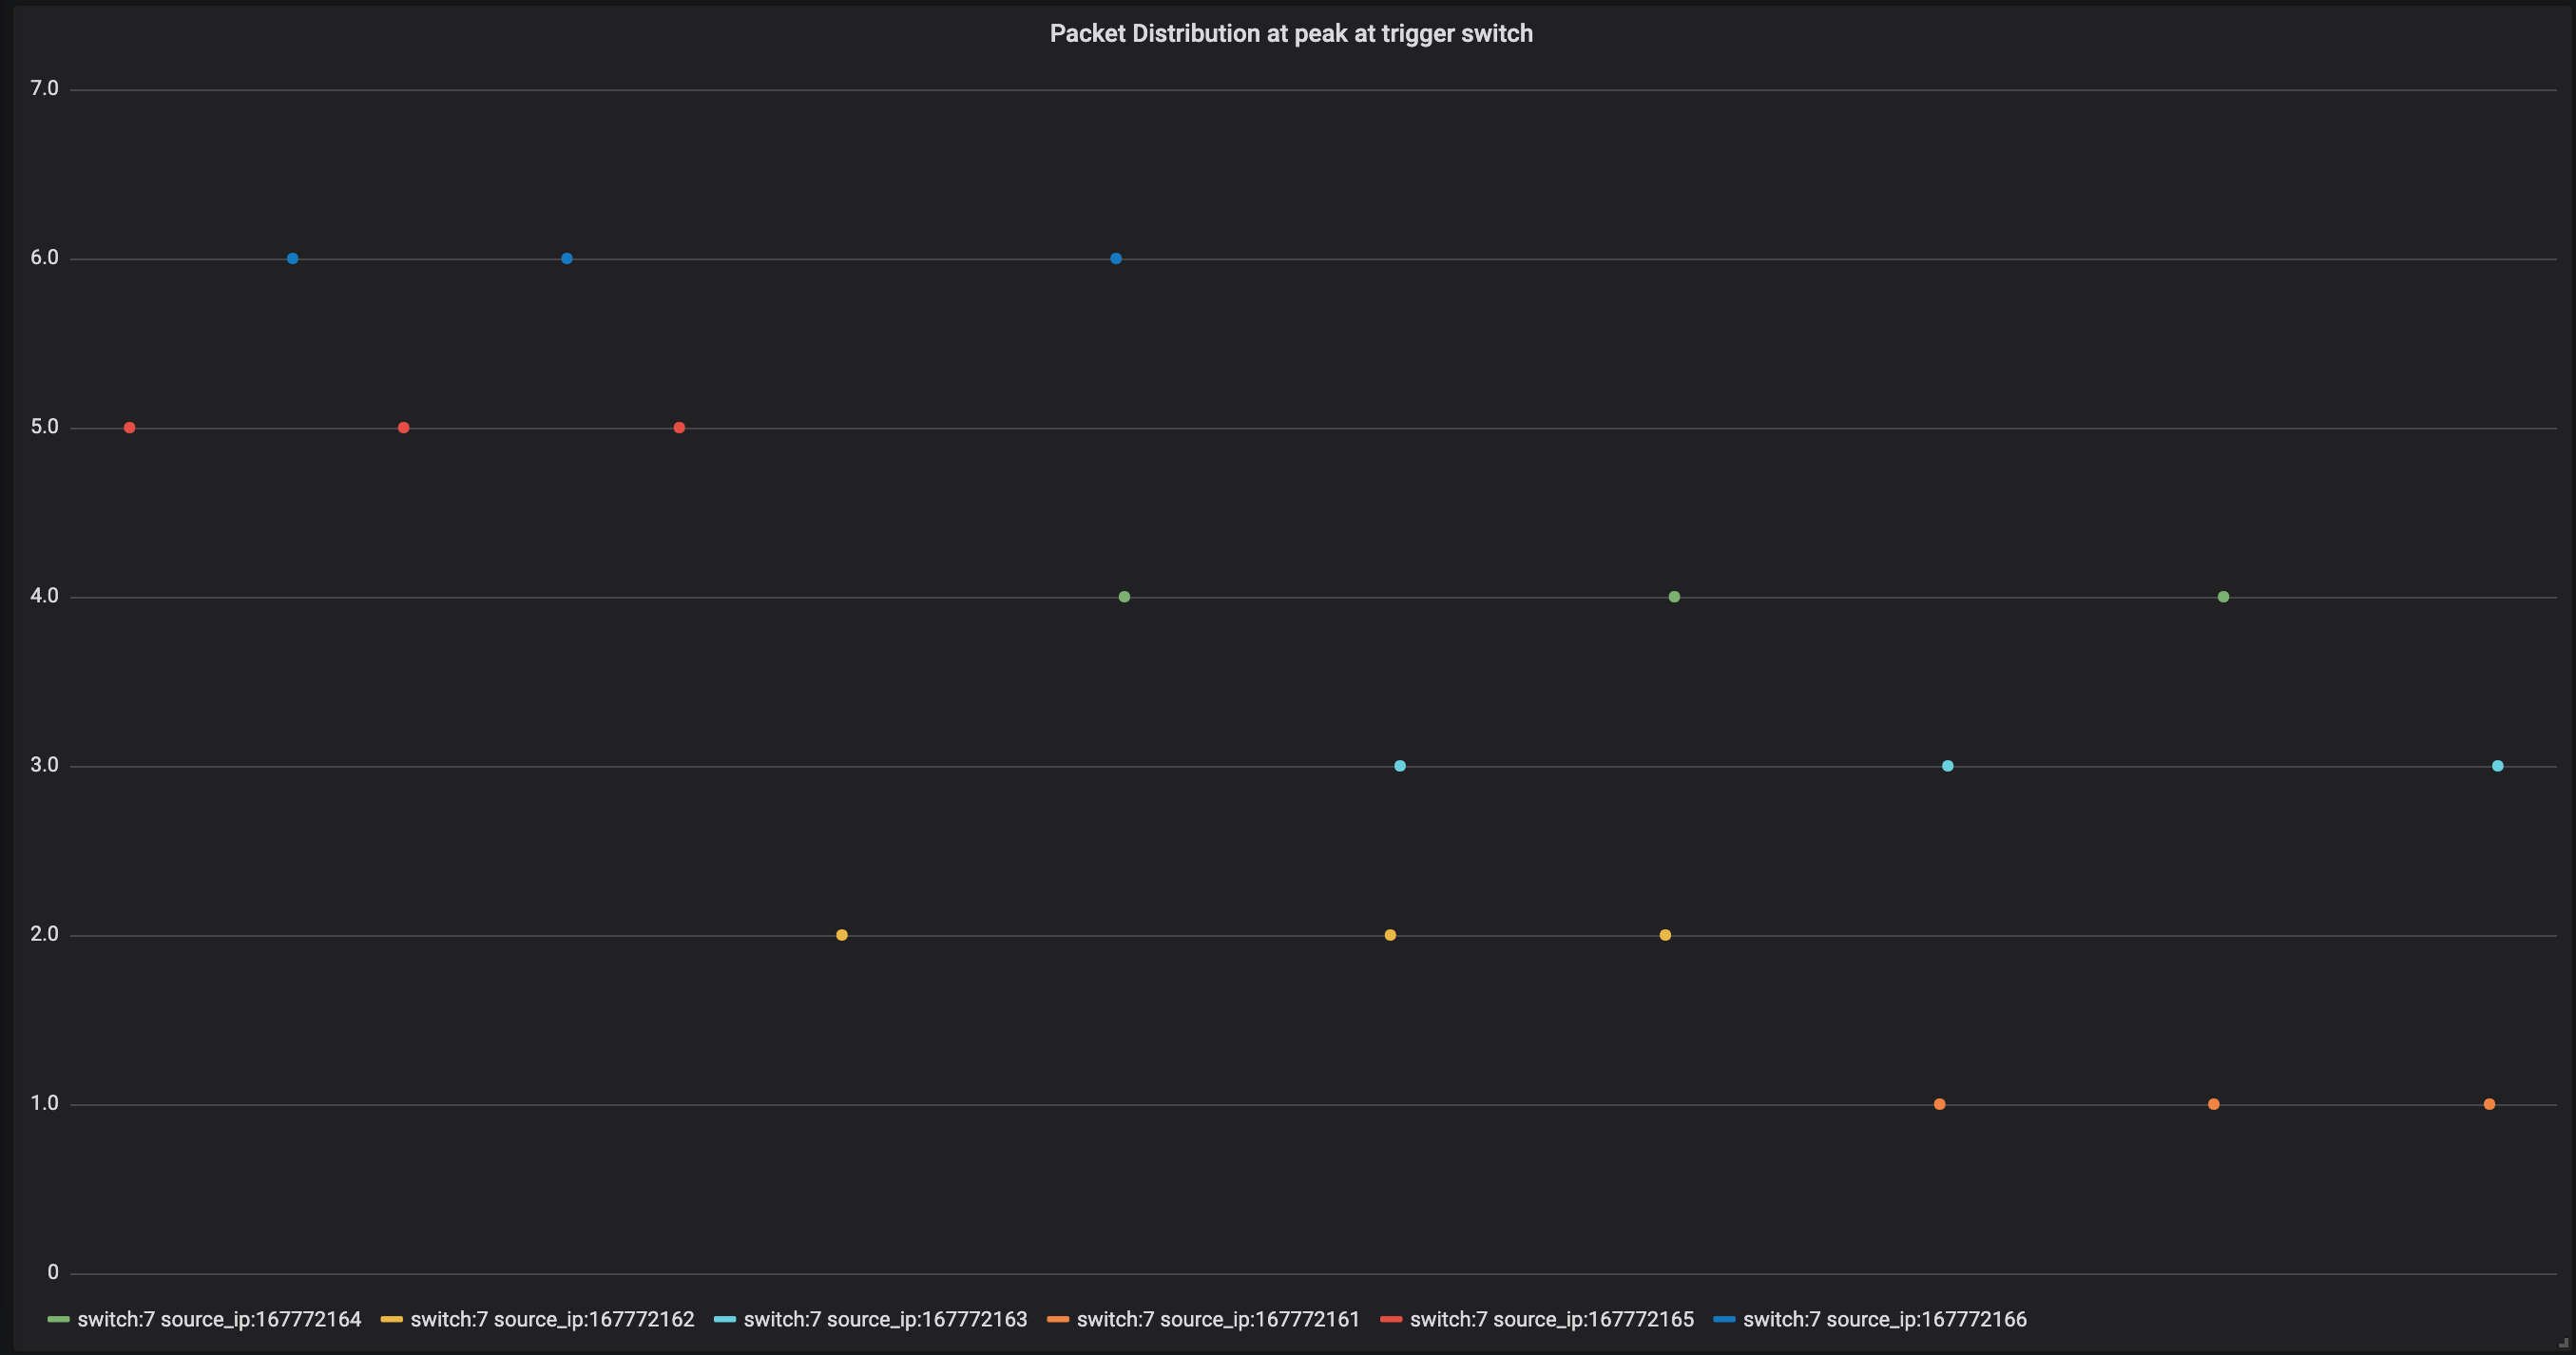
\includegraphics[width=1.0\columnwidth]{Figures/distribution_sync.png}
		\rule{35em}{0.5pt}
	\caption[Packet Distribution at Trigger Switch, Sync Incast]{Packet Distribution at Trigger Switch, Sync Incast. Note the highly even distribution.}
	\label{fig:distribution_sync}
\end{figure}

\section{Asynchronous Incast problem and Heavy Hitters}
\subsection{Description}
The Asynchronous Incast problem simply means a scenario where the queue depth increases over a period of microbursts
in the lack of any visible synchronization pattern. Often in these cases, we have the presence of a heavy hitter flow
(A flow which consumes a substantial amount of bandwidth that violates fairness) which causes congestion and overflowing
of buffers in switch.
\subsection{Configuration}
For creating an asynchronous incast scenario in our topology, we generate traffic of 1 Gbps from H1, H3, H4 and 6 Gbps from H6. The flow are routed
according to Figure \ref{fig:Synch Incast Topo} and get aggregated at switch 7.
\subsection{Diagnosis}
In cases of asynchronous incast with heavy hitters, we will see a single large peak in the plot of queue depth and usually a very
skewed distribution in the peak. The heuristic used here is similar to the one in synchronous incast except if the Jain's 
Fairness Index is less that 0.45, then it is classified as an asynchronous incast problem.
\subsection{Results and Illustrations}

The above heuristic was applied in 5 different scenarios of aynchronous incast of varied transmission rates.
The resultant values of Fairness Index calculated are given in table \ref{tab:J_Index_Async}.
\begin{table}[h]
	\begin{center}
	\begin{tabular}{ |p{3cm}|p{3cm}|  }
		\hline
		\multicolumn{2}{|c|}{Jain's Index} \\
		\hline
		Scenario & Value \\
		\hline
		1 & 0.469 \\
		2 & 0.362 \\
		3 & 0.383 \\
		4 & 0.418 \\
		5 & 0.403 \\
		\hline
	   \end{tabular}
	\end{center}
	
	\caption{Jain's Index Values for different scenarios of Asynchronous Incast}
	% Help
	\label{tab:J_Index_Async}
	\end{table}


Further, to help the network operator visualize the scenario, plots of link utilization and queue depth at 
trigger switch are plotted, along with packet distribution in the estimated peak, as shown in figures \ref{fig:link_utilization_async}, \ref{fig:queue_depth_async}
and \ref{fig:distribution_async}



\begin{figure}[htbp]
	\centering
		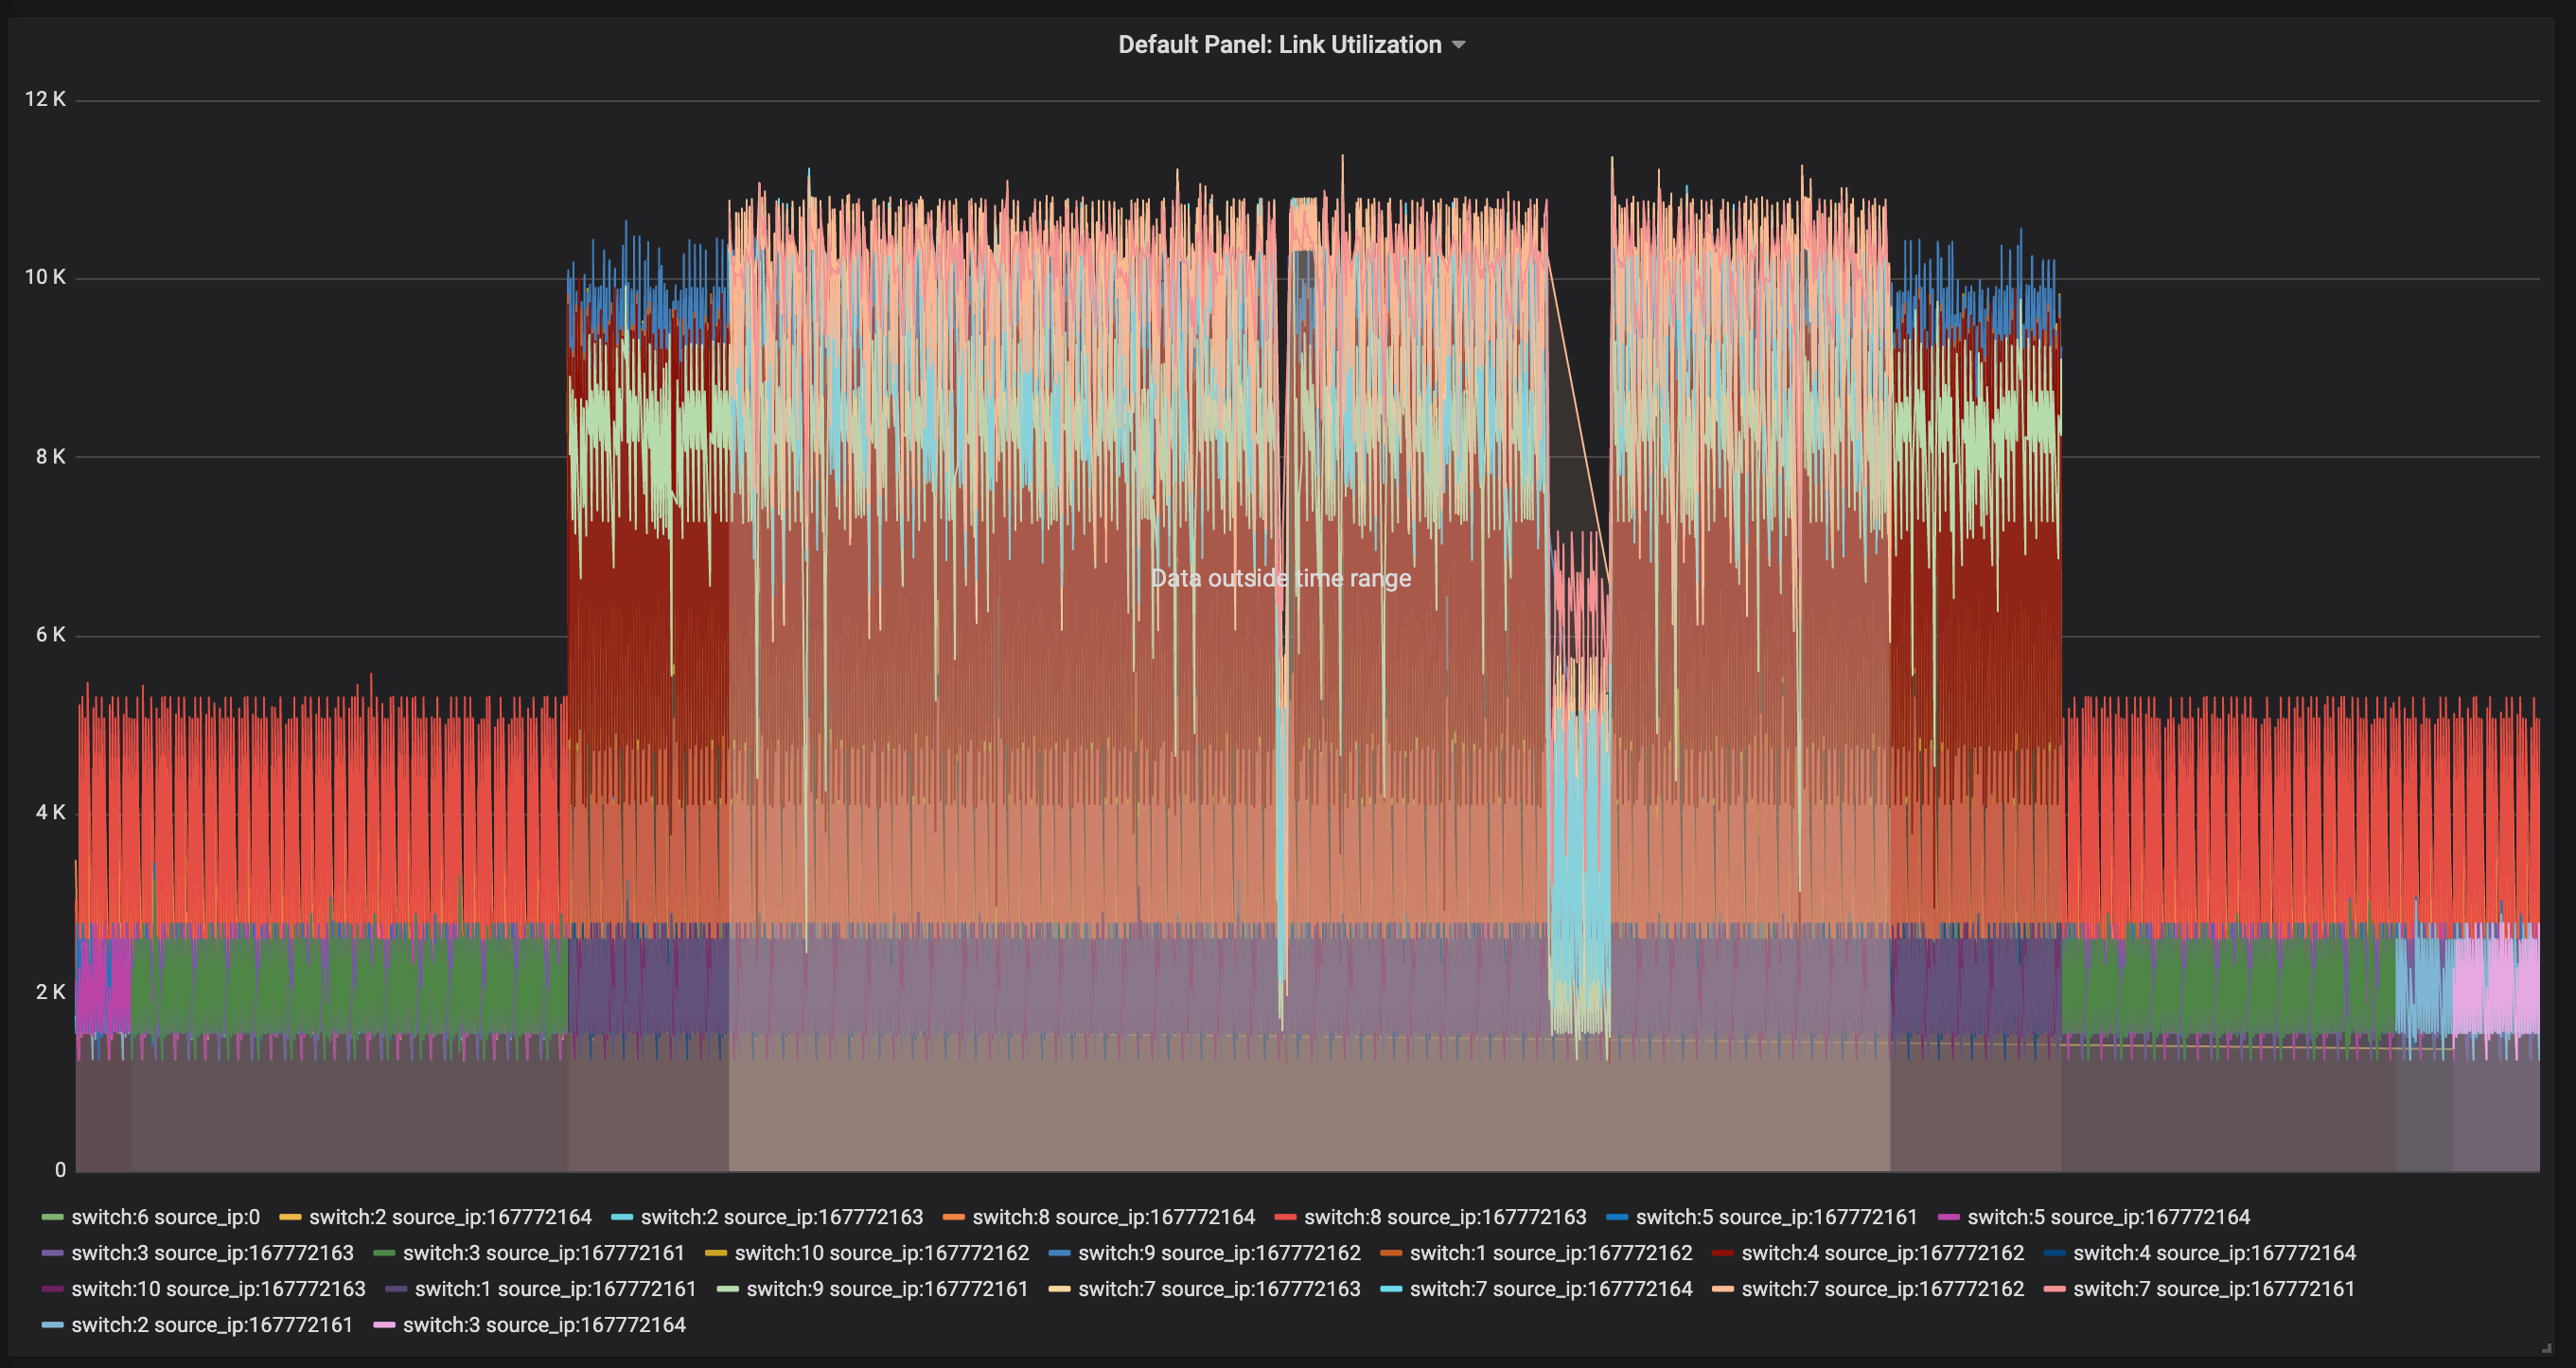
\includegraphics[width=1.0\columnwidth]{Figures/link_utilization_async.png}
		\rule{35em}{0.5pt}
	\caption[Link Utilization at Trigger Switch, Async Incast]{Link Utilization at Trigger Switch, Async Incast}
	\label{fig:link_utilization_async}
\end{figure}
\begin{figure}[htbp]
	\centering
		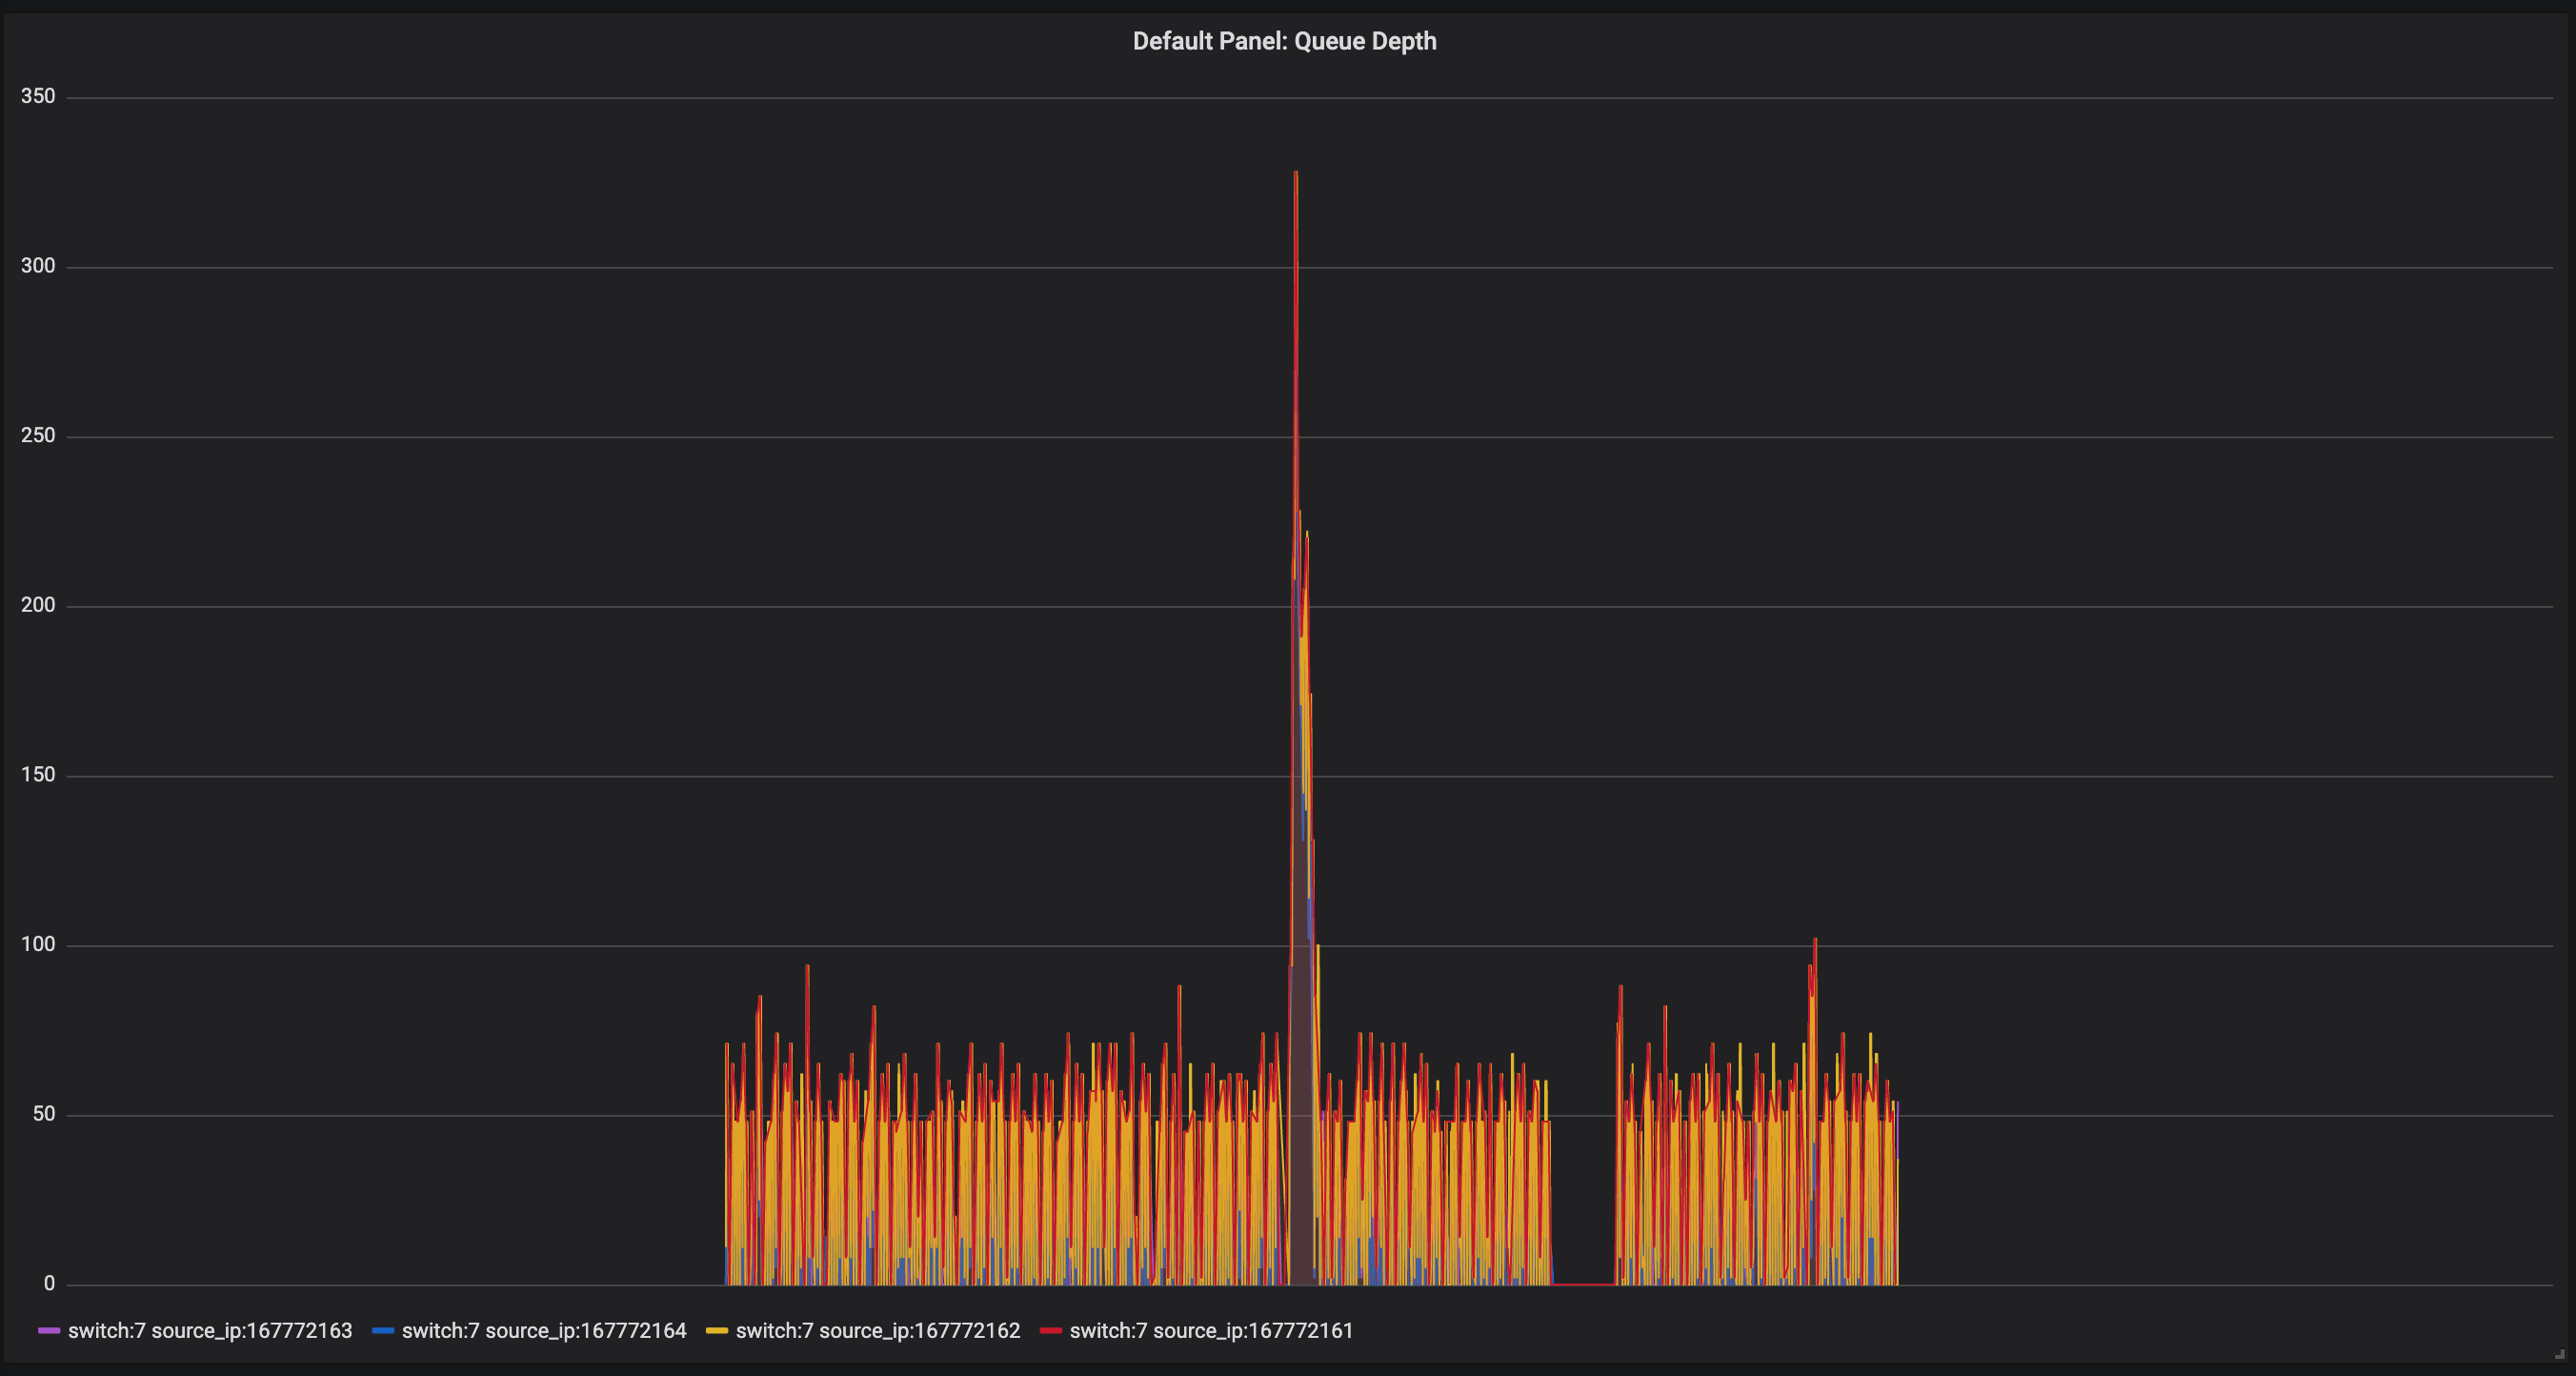
\includegraphics[width=1.0\columnwidth]{Figures/queue_depth_async.png}
		\rule{35em}{0.5pt}
	\caption[Queue Depth at Trigger Switch, Async Incast]{Queue Depth at Trigger Switch, Async Incast}
	\label{fig:queue_depth_async}
\end{figure}
\begin{figure}[htbp]
	\centering
		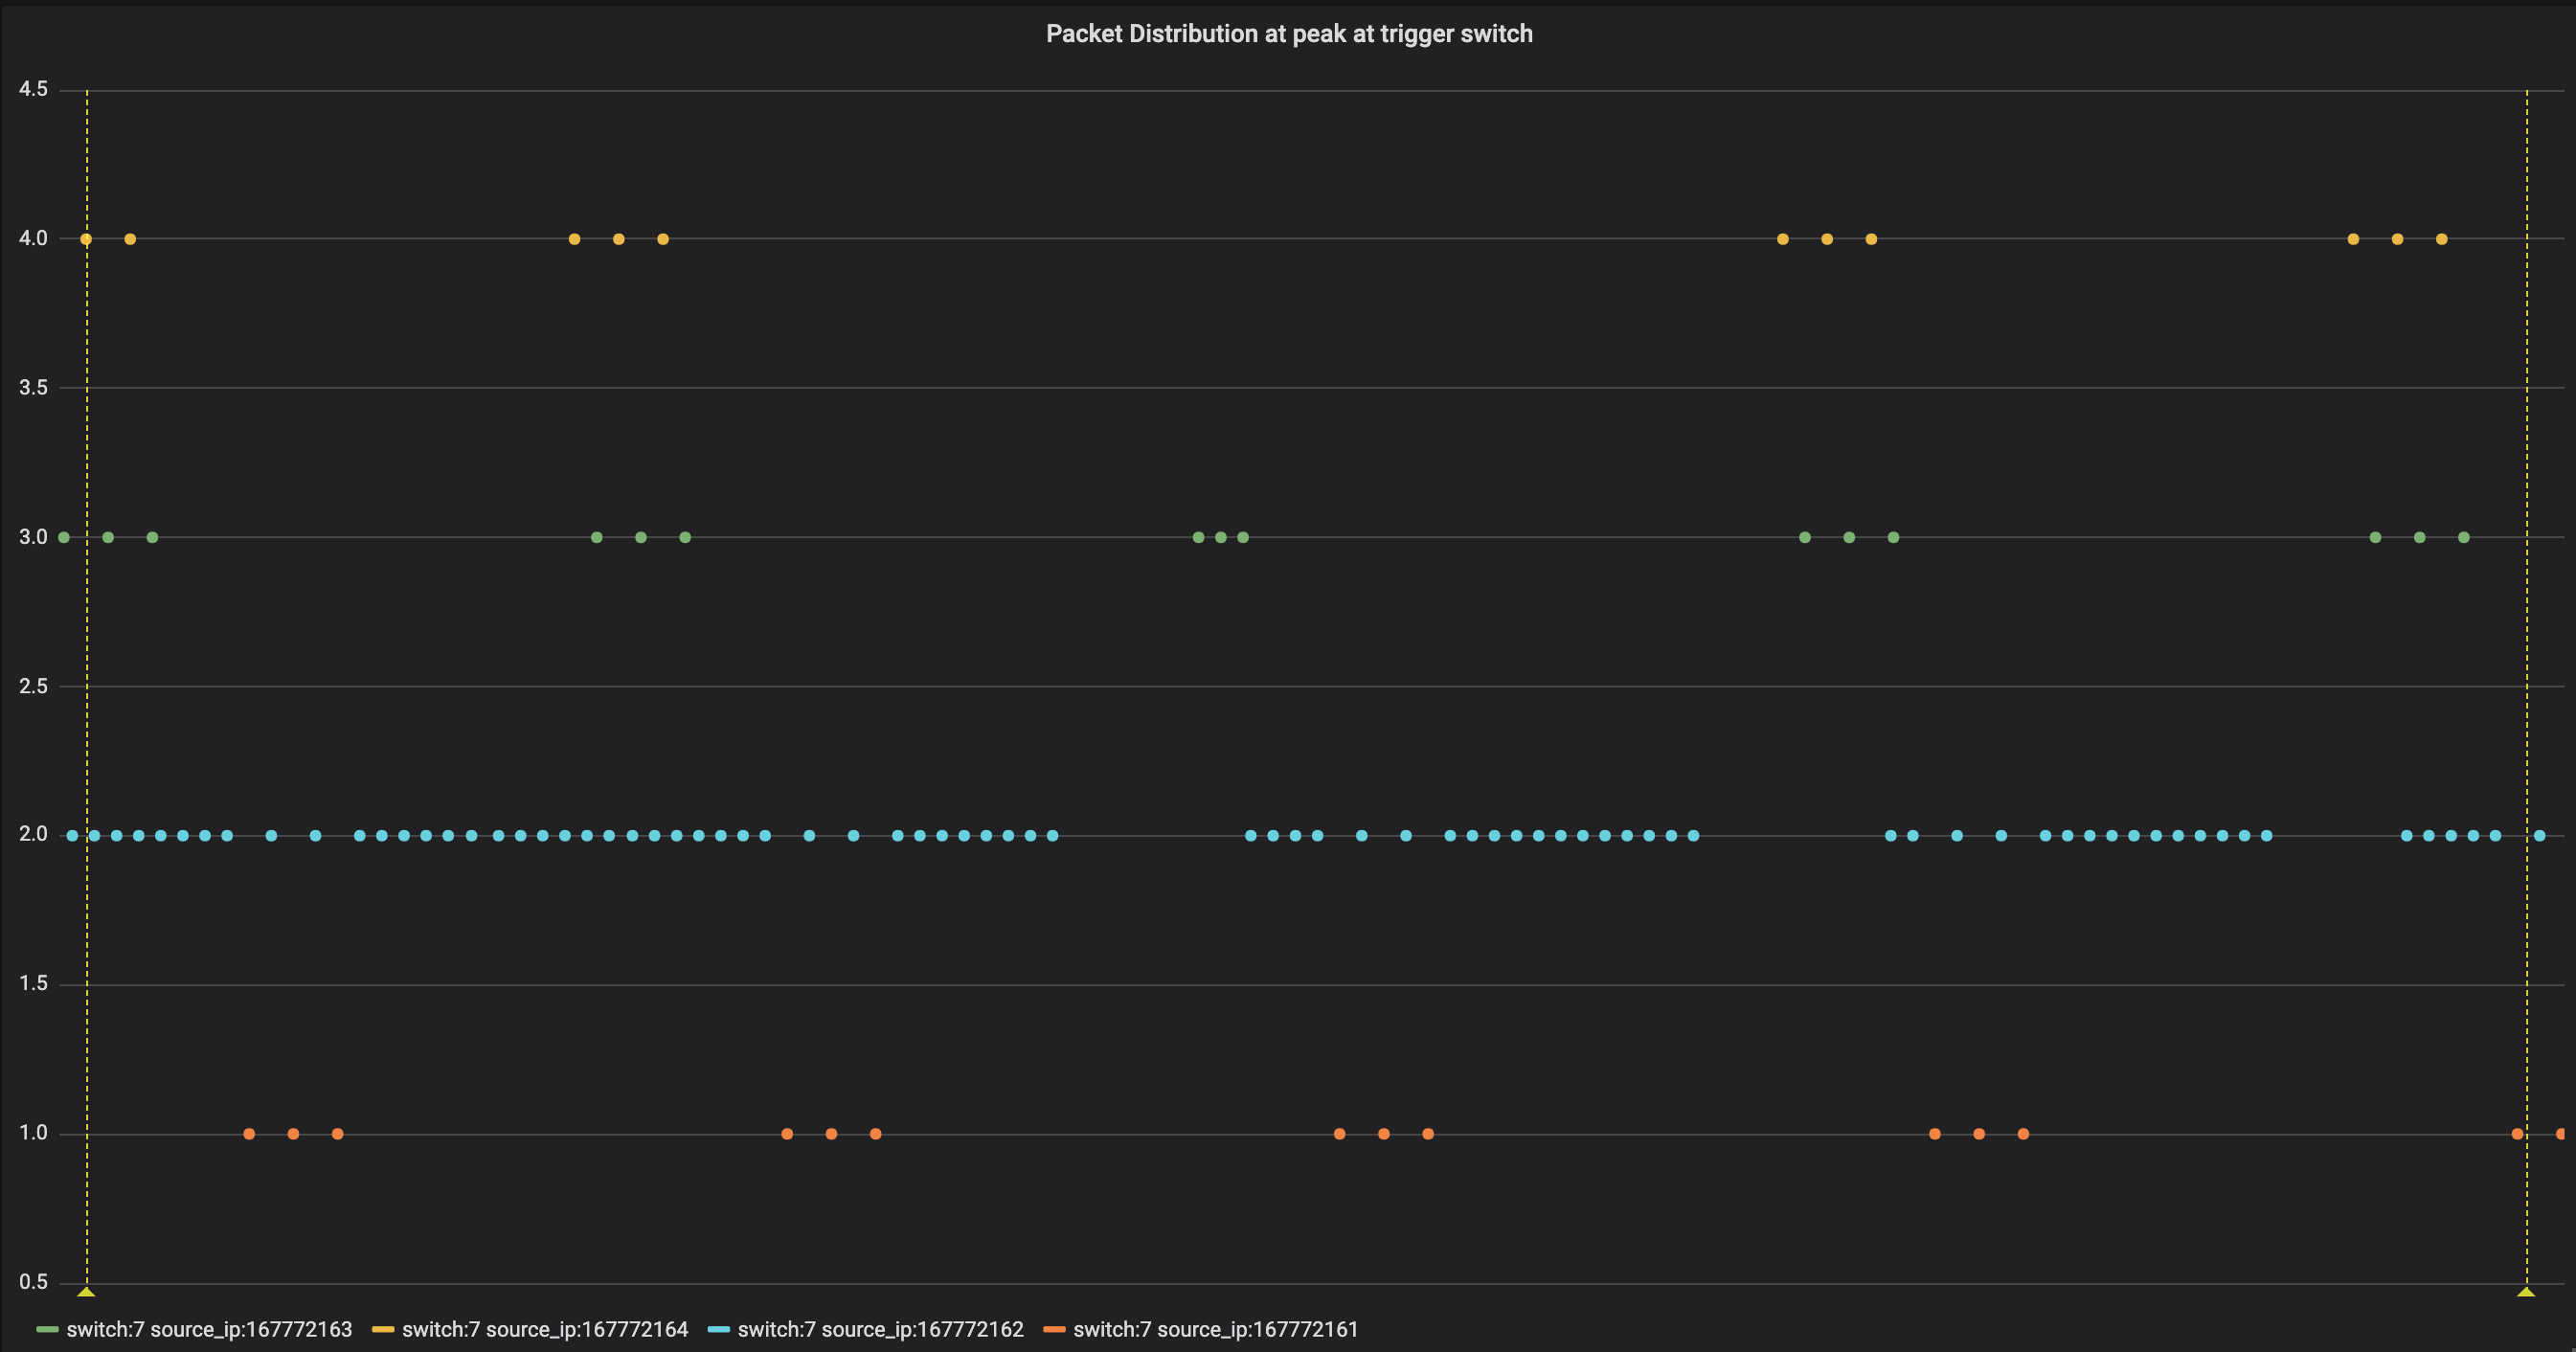
\includegraphics[width=1.0\columnwidth]{Figures/distribution_async.png}
		\rule{35em}{0.5pt}
	\caption[Packet Distribution at Trigger Switch, Async Incast]{Packet Distribution at Trigger Switch, Async Incast. Note the highly skewed distribution.}
	\label{fig:distribution_async}
\end{figure}


\section{Link Underprovisioning}
\subsection{Description}
A link underprovision occurs when the link is operating at near, or maximum capacity for prolonged periods of time (of the order of milliseconds or seconds).
This usually requires the operator to provide additional bandwidth for the link.
\subsection{Configuration}
For creating a link underprovision scenario in our topology, we generate traffic of 6 Gbps from H3, H4, H5 and 1 Gbps from H1 and H2. The flow are routed
according to Figure \ref{fig:Synch Incast Topo} and get aggregated at switch 7.
\subsection{Diagnosis}
As stated before, a link will be underprovisioned if it is overutilized for a duration of the order of milliseconds.
If we find that the width of the peak as found in Algorithm 1 is of the order of milliseconds, and that the link is being overutilized, say by setting a threshold
to be average utilization greater than 0.8 * max capacity, then we classify the link to be overutilized.
\subsection{Results and Illustrations}
The above heuristic was applied to 2 different scenarios of link underprovision of varied transmission rates.
The resultant values of peak width calculated are given in table \ref{tab:Peak_Width}
\begin{table}[h]
\begin{center}
\begin{tabular}{ |p{3cm}|p{5cm}|  }
	\hline
	\multicolumn{2}{|c|}{Peak Width} \\
	\hline
	Scenario & Duration (in microseconds) \\
	\hline
	1 & 2575.626 \\
	2 & 4713.071 \\
	\hline
   \end{tabular}
\end{center}

\caption{Peak Width Duration for different scenarios of Link Underprovisioning}
% Help
\label{tab:Peak_Width}
\end{table}

Further, to help the network operator visualize the scenario, plots of link utilization and queue depth at 
trigger switch are plotted, along with packet distribution in the estimated peak, as shown in figures \ref{fig:link_utilization_under}, \ref{fig:queue_depth_under}
and \ref{fig:distribution_under}

\begin{figure}[htbp]
	\centering
		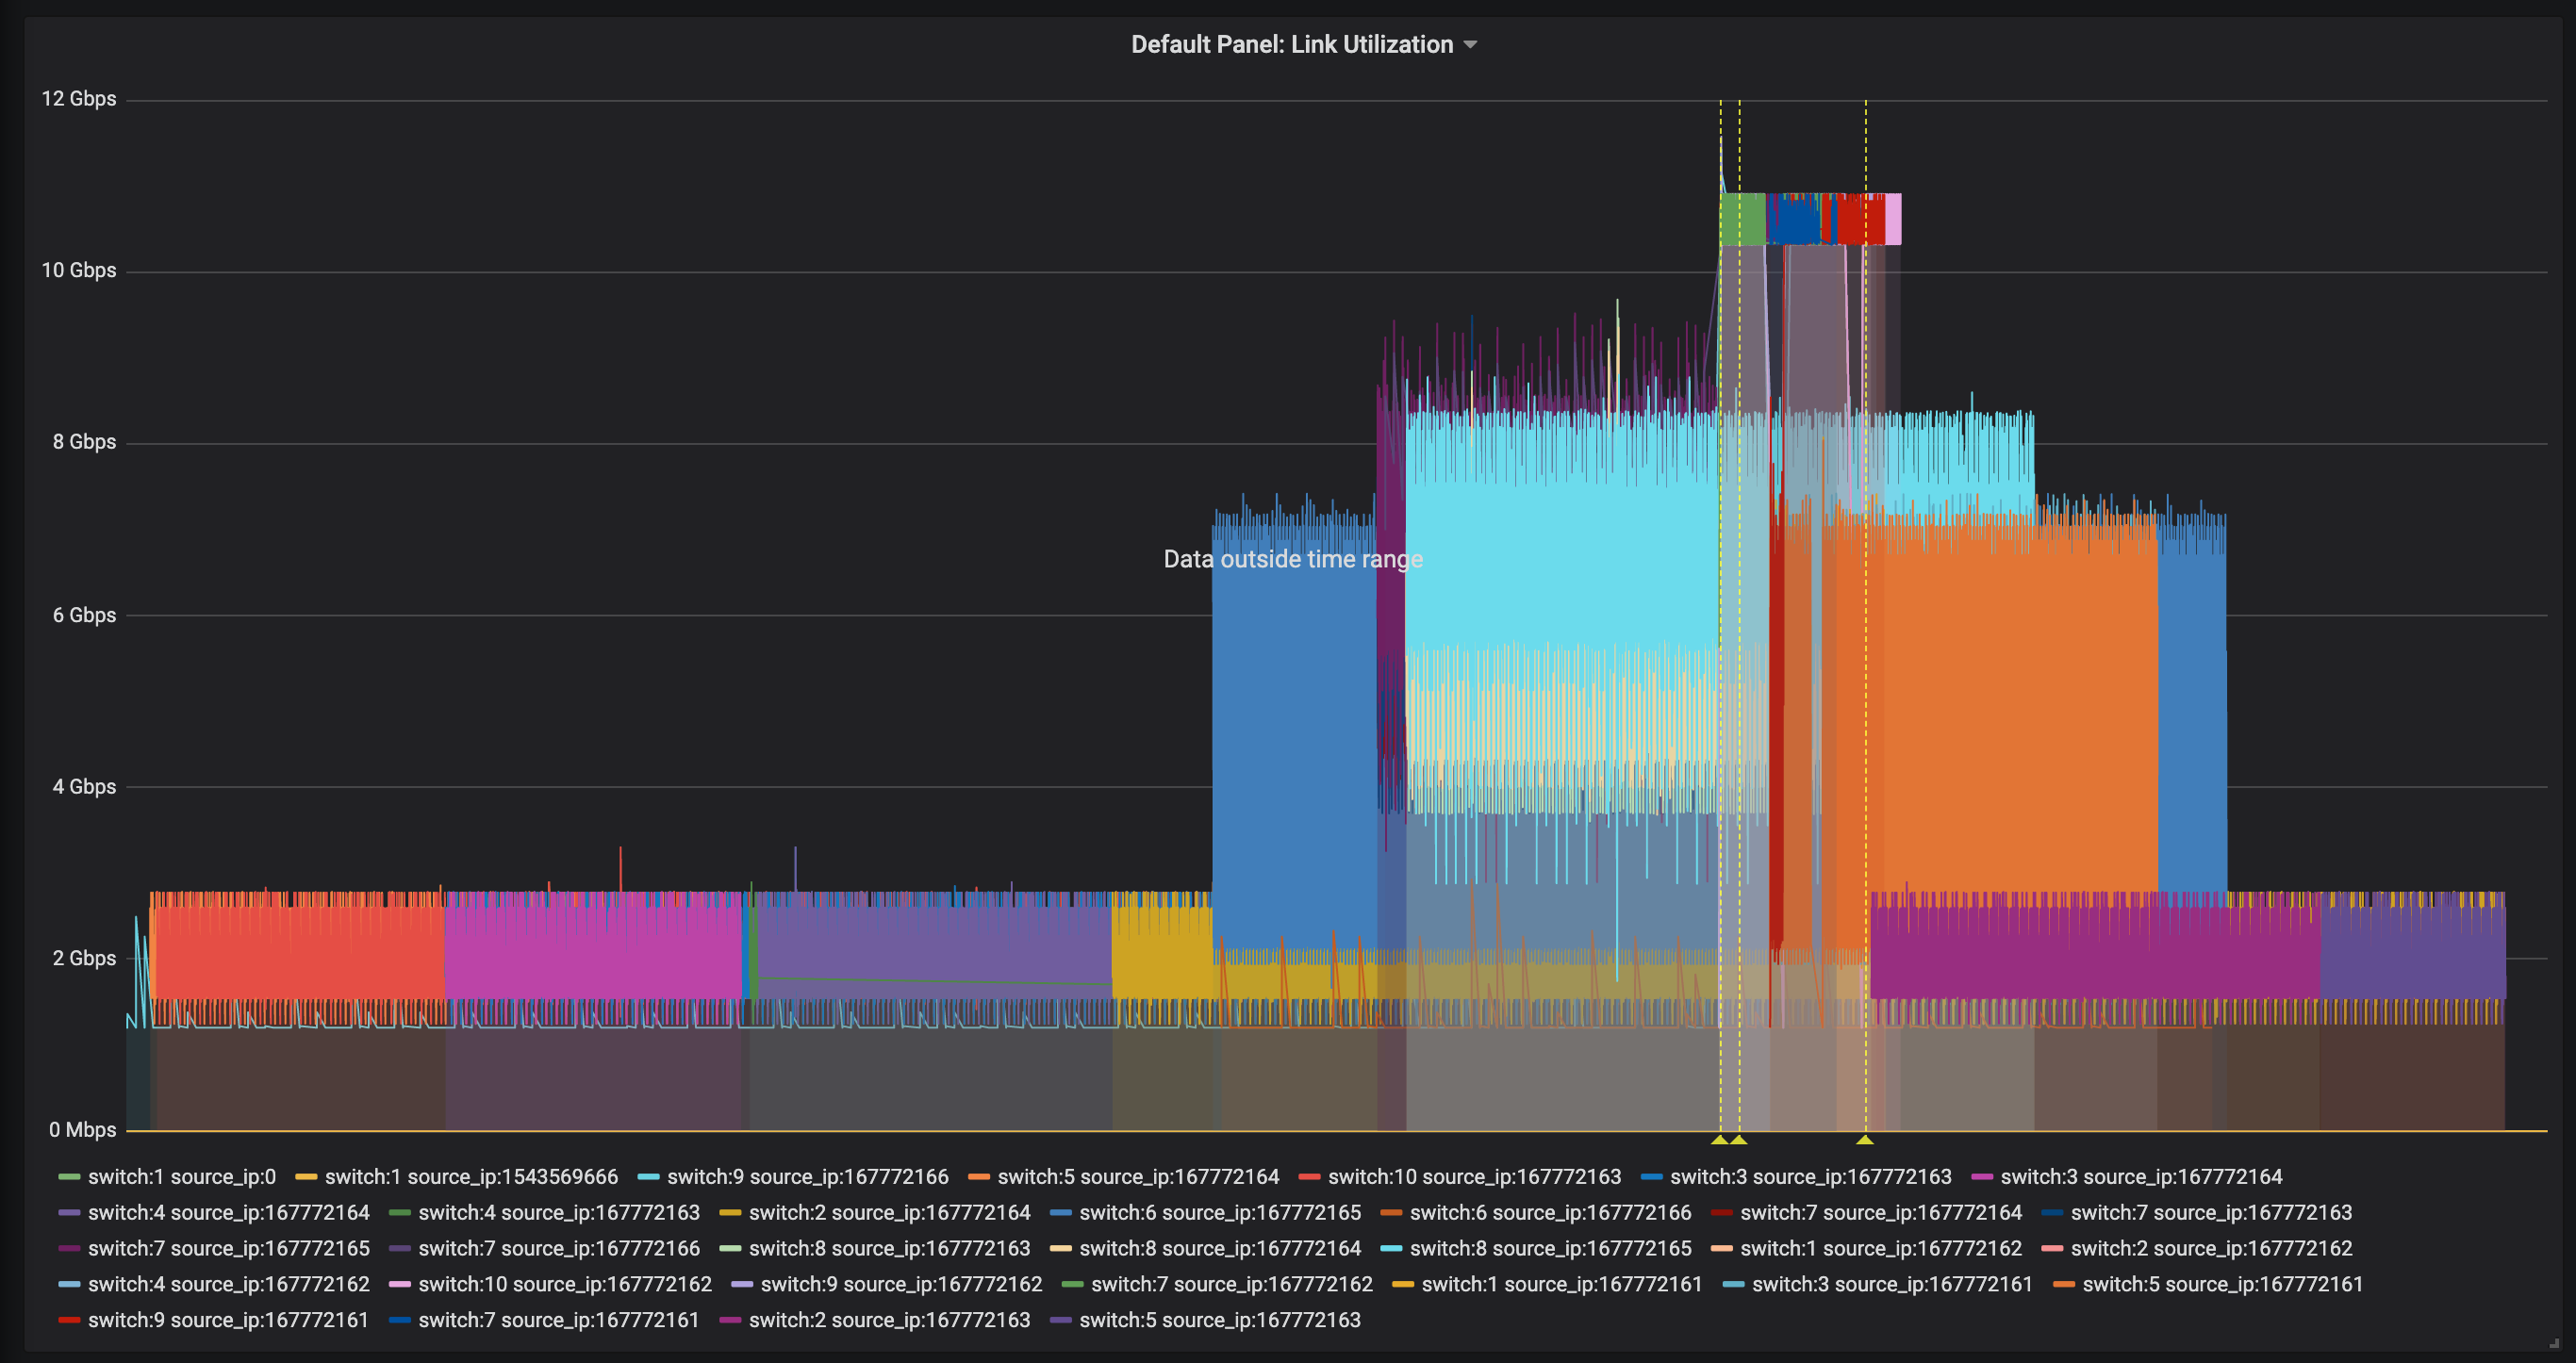
\includegraphics[width=1.0\columnwidth]{Figures/link_utilization_under.png}
		\rule{35em}{0.5pt}
	\caption[Link Utilization at Trigger Switch, Link Underprovisioning]{Link Utilization at Trigger Switch, Link Underprovisioning}
	\label{fig:link_utilization_under}
\end{figure}
\begin{figure}[htbp]
	\centering
		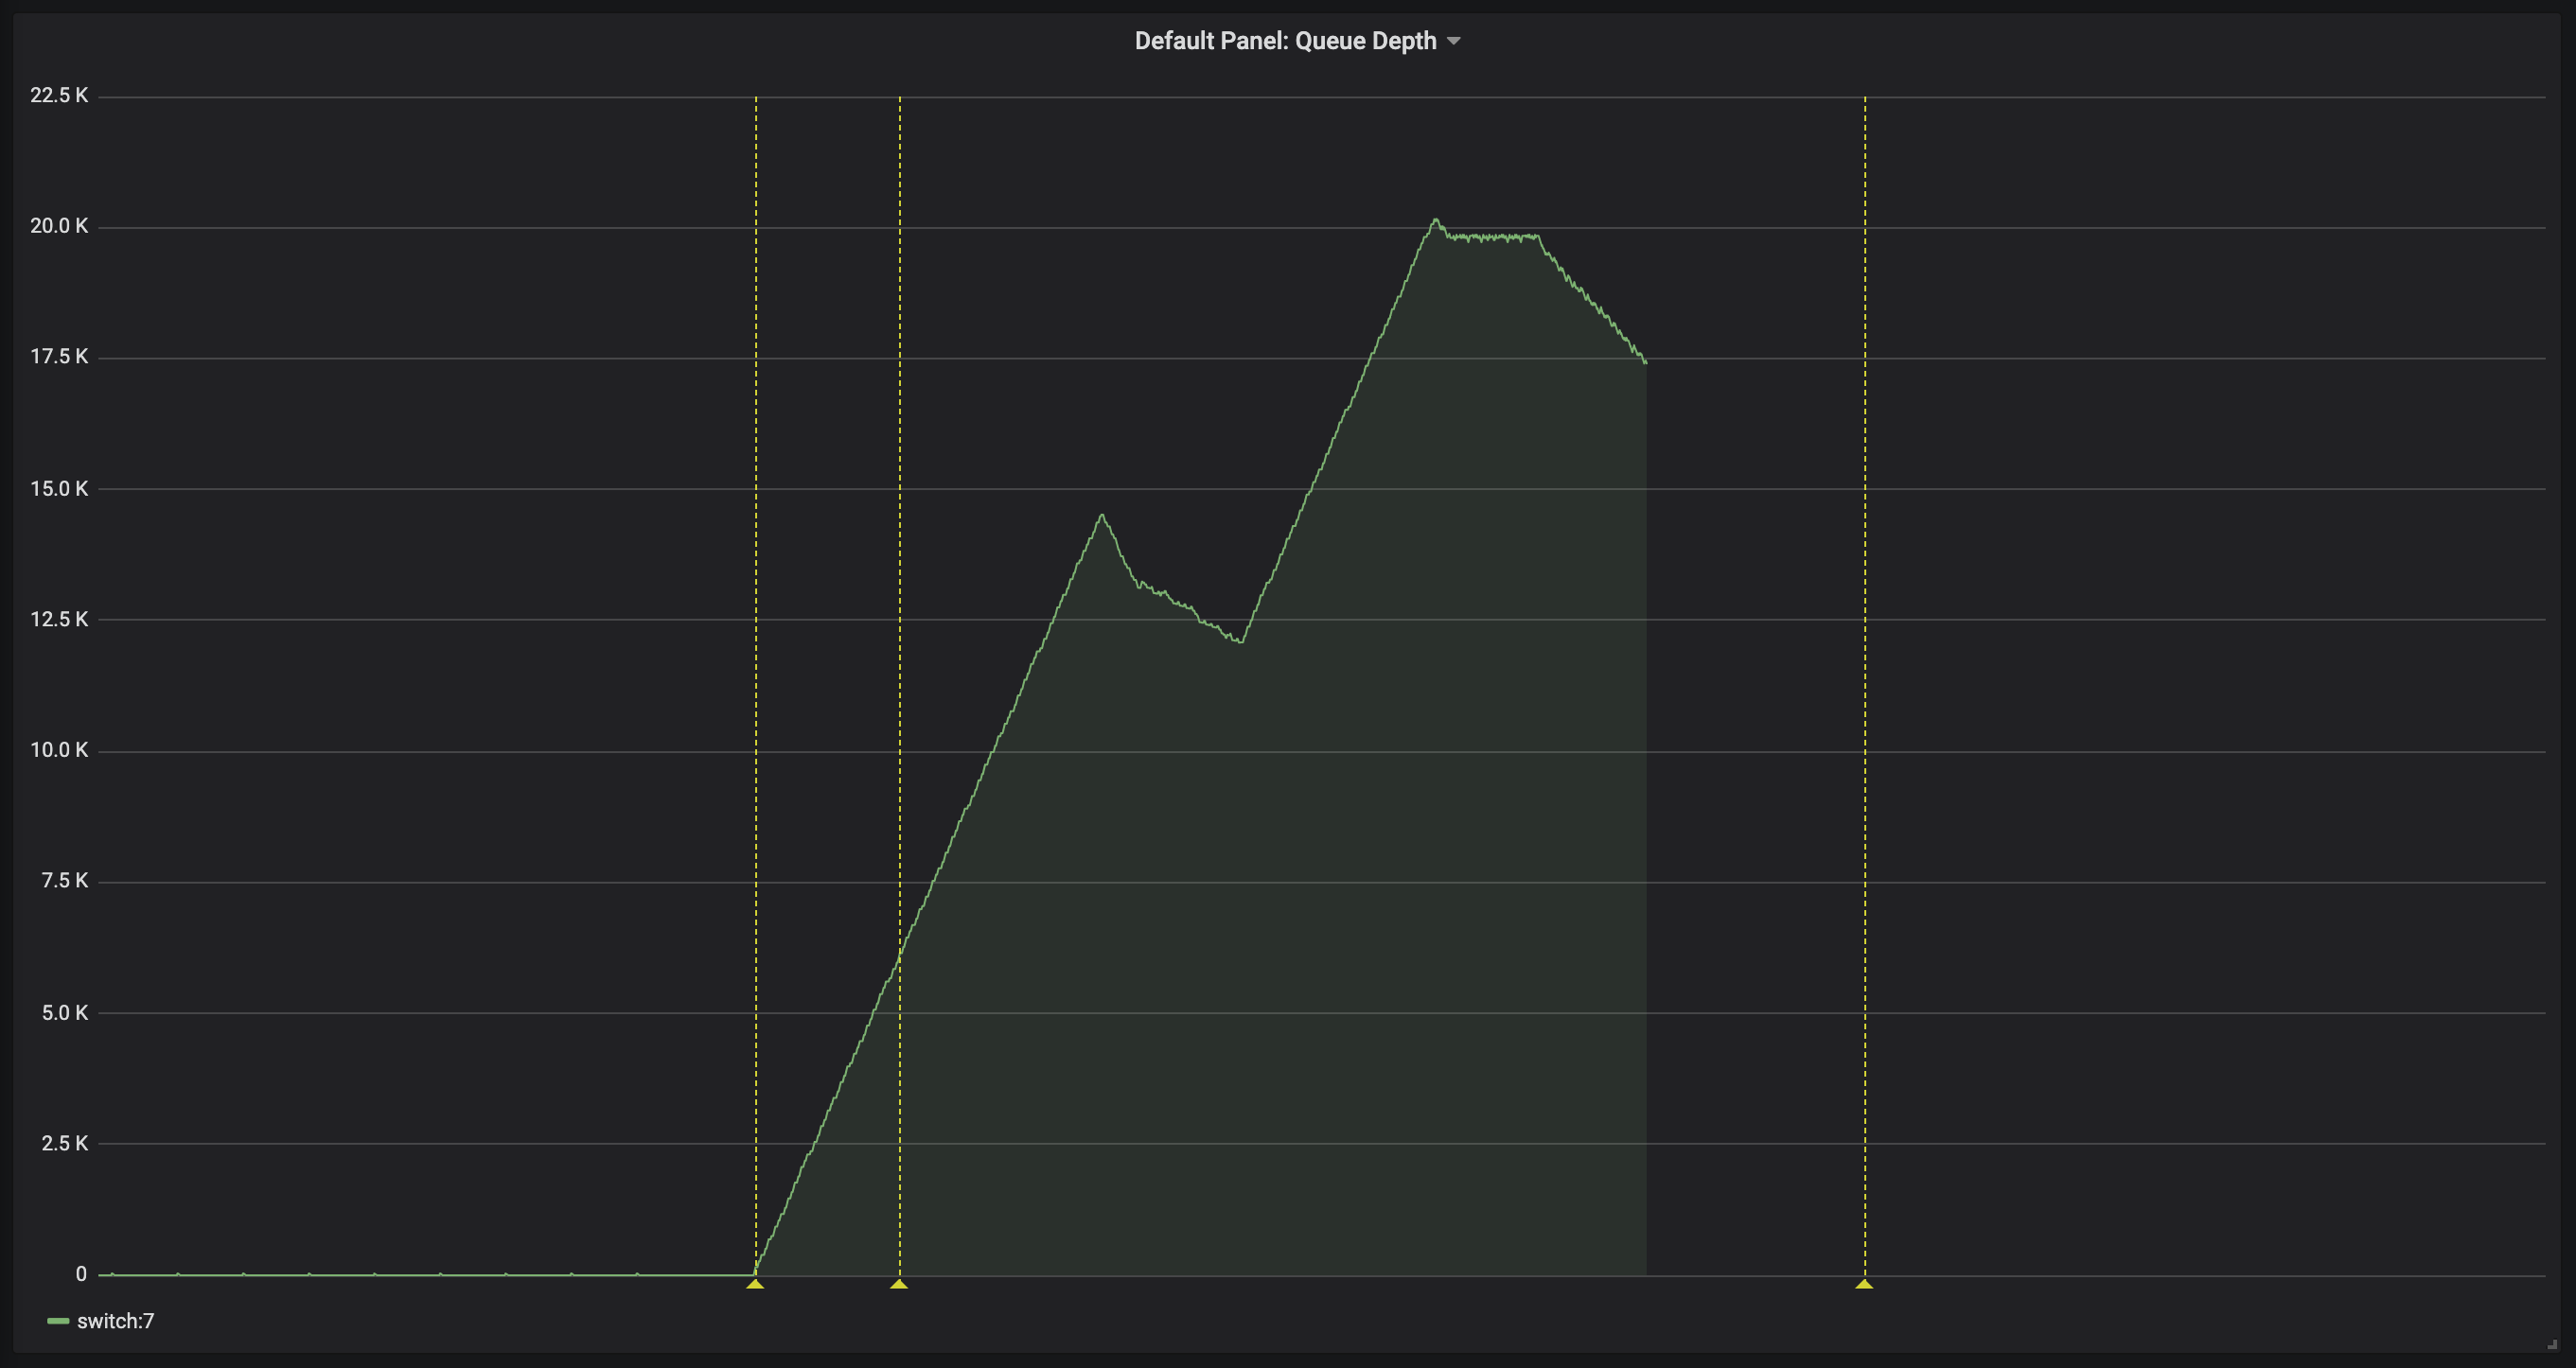
\includegraphics[width=1.0\columnwidth]{Figures/queue_depth_under.png}
		\rule{35em}{0.5pt}
	\caption[Queue Depth at Trigger Switch, Link Underprovisioning]{Queue Depth at Trigger Switch, Link Underprovisioning}
	\label{fig:queue_depth_under}
\end{figure}
\begin{figure}[htbp]
	\centering
		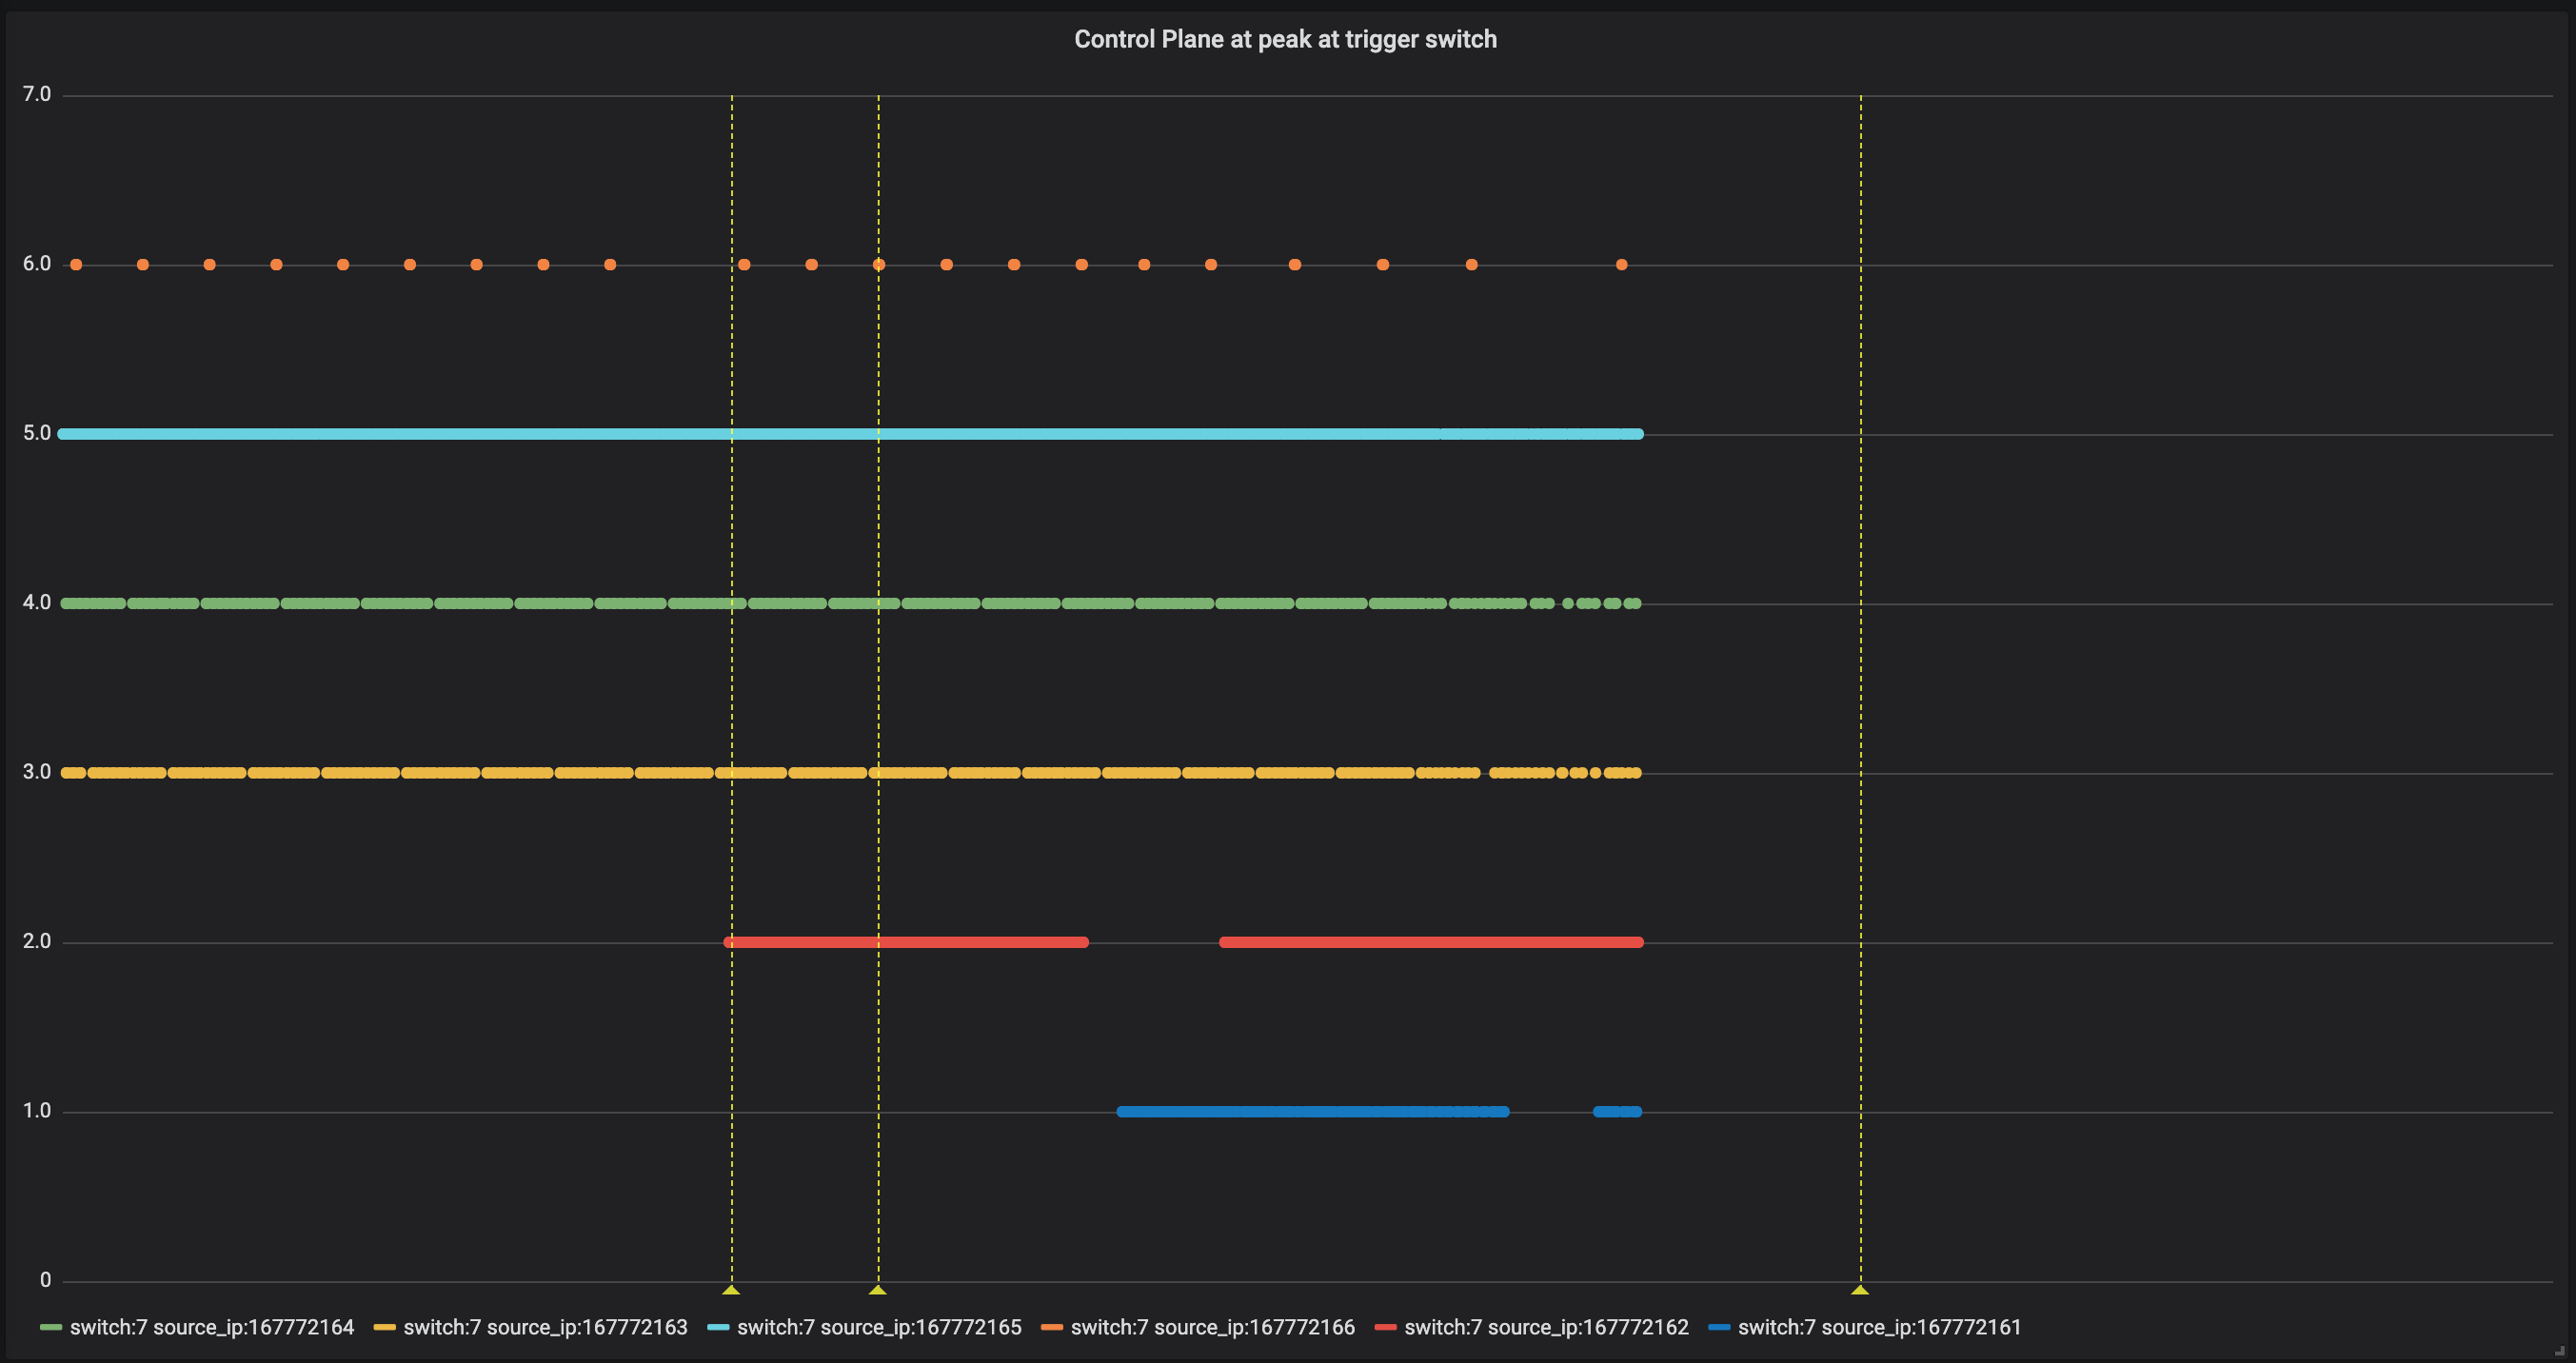
\includegraphics[width=1.0\columnwidth]{Figures/distribution_under.png}
		\rule{35em}{0.5pt}
	\caption[Packet Distribution at Trigger Switch, Link Underprovisioning]{Packet Distribution at Trigger Switch, Link Underprovisioning. Note the overlapping dots, showing link to be overutilized.}
	\label{fig:distribution_under}
\end{figure}
\section{Conclusions and further scope}

Based on the reasoning done in the preceding sections, a unified scheme to classify arbitrary scenarios based on the above discussion would be as follows:
\begin{itemize}
	\item Estimate the peak width in the graph
	\item If it is more than 1 millisecond, check if link is being overutilized. If so, it is probably a case of link underprovisioning.
	\item If it is less than 1 microsecond, calculate Jain's Fairness Index of packet distribution. If it is greater than 0.7, it is probably a synchronized incast. 
	\item Else, if it is less than 0.45, it is probably an asynchronous incast with heavy hitters present.
	\item Else (it is between 0.45 and 0.7), plot appropriate graphs for queue depth and link utilization and let the network operator deduce the exact problem.
\end{itemize}

As I further pursue my thesis, my goal is to isolate many such problems (two problems I currently have in mind are link failure 
and change of control plane policy), diagnose them on an individual basis, and at the end consolidate everything together into a single unified logic for diagnosing 
varied faults in a network.